\documentclass[11pt,a4paper]{article}
\usepackage{times,latexsym}
\usepackage[T1]{fontenc}
\usepackage[utf8]{inputenc}
\usepackage{url}
\usepackage[]{tacl2021v1}
\usepackage{graphicx}
\usepackage{amsmath,amssymb}
\usepackage{booktabs}
\usepackage{array}
\usepackage{tabularx}
\usepackage{longtable}
\usepackage{calc}
\usepackage{capt-of}
\usepackage[section]{placeins}
\usepackage{balance}

\newcommand{\tightlist}{}
\allowdisplaybreaks
\setlength{\dbltextfloatsep}{8pt plus 1pt minus 2pt}
\setlength{\dblfloatsep}{8pt plus 1pt minus 2pt}
\setlength{\textfloatsep}{8pt plus 1pt minus 2pt}
\setlength{\floatsep}{8pt plus 1pt minus 2pt}
\setlength{\abovecaptionskip}{4pt plus 1pt minus 1pt}
\setlength{\belowcaptionskip}{2pt plus 1pt minus 1pt}
\renewcommand{\topfraction}{0.95}
\renewcommand{\dbltopfraction}{0.95}
\renewcommand{\textfraction}{0.05}
\renewcommand{\floatpagefraction}{0.85}
\renewcommand{\dblfloatpagefraction}{0.85}
\makeatletter
\setlength{\@fptop}{0pt}
\setlength{\@fpsep}{8pt plus 1fil}
\setlength{\@fpbot}{0pt plus 1fil}
\setlength{\@dblfptop}{0pt}
\setlength{\@dblfpsep}{8pt plus 1fil}
\setlength{\@dblfpbot}{0pt plus 1fil}
\makeatother
\raggedbottom

\title{Denominator-Explicit Reporting for Target-Aware LLM Interventions under Refusal Censoring}
\author{}
\date{}

\begin{document}
\maketitle
\begin{abstract}
Target-aware LLM evaluations often report ``success rates'' only after an advising model has generated a response. When refusals remove both the intervention and the downstream decision, this convention changes the estimand: it measures a selected generated subset, not exposure across all attempts. We introduce denominator-explicit reporting for refusal-censored decision shift. The framework separates generation availability, realized exposure on a common denominator, generated-subset conditional shift, and post-hoc tactic audits. In a fixed case study of 2,968 attacker--defender evaluation instances, a single deterministic evaluation yields 72.7\% generated-subset conditional target shift, 12.4\% realized exposure on the full denominator, and 0.0\% observed exposure under a policy-framing self-gate. A human validation sample of 360 instances showed high refusal-label agreement, and option extraction agreed exactly among sampled generated observations. Tactic labels were less stable: pre-adjudication agreement was limited for strict-deception labels (Cohen's \(\kappa=0.403\)) and near chance for a broader misleading-tactic label (\(\kappa=0.040\)). The tactic labels therefore support validation-sample audit counts, not prevalence estimates. The contribution is a reporting rule for refusal-censored target-aware evaluations: state the generation process, denominator, measurement label, and identification boundary before interpreting any rate.
\end{abstract}

\section{Introduction}\label{introduction}


Target-aware large language model (LLM) evaluations increasingly study whether an advising model can move a downstream decision toward a specified target \citep{TanEtAl2025DuETPD,HwangEtAl2025TrickGrader,LiuEtAl2025}. We formalize this advising model as the attacker in an attacker--defender pair. A common reporting shortcut is to compute a single ``success rate'' only among cases where the attacker generates a response. That shortcut leaves refusals outside the denominator. When the attacker refuses to generate a target-aware message, the downstream defender decision is unobserved. We call this refusal censoring: denominator choice becomes part of the estimand, not a formatting detail \citep{HuangEtAl2025DeceptionBench,WuEtAl2025OpenDeception,ChernEtAl2024BeHonest}.

A single generated-only rate collapses three quantities. Generation availability asks whether a usable intervention is produced at all. Generated-subset conditional target shift asks what happens after generation has occurred. Realized exposure asks whether the observed full pathway both generates an intervention and moves a non-target baseline decision to the attacker target. The same evaluation can therefore yield a high conditional shift rate among generated cases, a much smaller realized exposure rate on a common denominator, and zero observed exposure when a more stringent self-gate blocks generation. These are not competing estimates of one fact; they answer different questions.

We focus on the measurement problem that precedes deployment, human-persuasion, deception-prevalence, intent, or target-specific causal claims. If target-aware generation is refused, the downstream target-aware decision is unobserved. Generated-only conditional rates and full-denominator exposure rates therefore answer different questions.

The distinction matters in policy, finance, and ethics settings, where a single objective correctness label is often absent. In these scenarios, the directly observable outcome is a paired decision contrast---a decision shift---rather than movement toward a factual truth. Post-hoc tactic labels require an additional audit layer. Claims of strict deception require separate, verifiable evidence of explicit falsehood, fabrication, or false attribution \citep{Hagendorff2024DeceptionAbilities,SuEtAl2025AILieDar,HuangEtAl2025DeceptionBench}. The framework therefore keeps observable decision shift separate from audited tactic labels whose reliability must itself be measured.

The case study below shows why this separation is practical, not just conceptual. In the rerun tactic audit, pre-adjudication strict-label agreement was limited, and broad-codebook agreement was near chance. Tactic labels are therefore validation targets, not stable ground truth to fold into the primary outcome. Refusal censoring adds a second boundary: after a refusal, the downstream defender decision is unobserved, so estimating the counterfactual outcome for refused cases requires assumptions that the observed data alone cannot validate \citep{Heckman1979,Vella1998,Manski1990}.


We address these issues with a denominator-explicit, three-branch reporting design. For each evaluation instance---a scenario crossed with an ordered attacker--defender model pair---the protocol records an independent baseline decision, a target-unaware advice decision, and a target-aware pathway observed only when the attacker generates an intervention. It measures generation availability under prompt-conditional self-gates and audits generated texts for deception markers, while keeping those labels separate from the primary decision-shift outcome. This separation aligns with causal text analysis principles that keep text interventions, downstream outcomes, and measurement labels distinct \citep{KeithEtAl2020TextCausal,FederEtAl2022CausalNLP,EgamiEtAl2022TextCausal}.

We instantiate the design in a case study of 2,968 evaluation instances. The study shows a large denominator-driven contrast between generated-subset conditional target shift (72.7\%) and realized exposure on the full denominator (12.4\%), and it shows that strict-deception labels need reliability evidence before they can support prevalence claims. The paper makes three methodological contributions: (i) an estimand taxonomy that separates generation availability, realized exposure, generated-subset conditional shift, and partial-identification bounds; (ii) a measurement protocol that keeps observable decision shift separate from post-hoc tactic labels; and (iii) a reporting rule that requires the generation process, denominator, measurement label, and identification boundary to be stated before any reported rate is interpreted. The underlying selection principle is standard; the contribution is its transfer to refusal-censored target-aware LLM evaluation and its operationalization as a reusable reporting contract.

\section{Related work}\label{related-work-the-measurement-gap}

Prior work shows that LLM outputs can alter decisions, exhibit deceptive or dishonest behavior under some conditions, and refuse unsafe or policy-sensitive requests. The measurement gap addressed here is different: existing evaluations often do not keep the denominator fixed when a target-aware intervention is refused or otherwise unavailable. As a result, generated-subset ``success'' can be mistaken for full-pathway exposure, and decision shift can be conflated with deception.

\subsection{Decision shift is not correctness}\label{decision-change-rather-than-correctness}

Persuasion and decision-influence benchmarks already move beyond one-shot accuracy. DuET-PD studies stance-change dynamics in persuasive dialogue, and adversarial-persuasion work shows that style can alter LLM-judge decisions even when correctness should be invariant to presentation \citep{TanEtAl2025DuETPD,HwangEtAl2025TrickGrader,durmus2024measuring}. Our estimand differs in three ways: the unit is a one-turn contrast between an independently measured baseline decision \(Y_i^{base}\) and a target-aware decision \(Y_i^{tgt}\); the target \(T_i\) is benchmark-defined rather than necessarily true or false; and refusal makes \(Y_i^{tgt}\) unobserved rather than merely unfavorable.

This framing is adjacent to sycophancy and LLM-as-judge robustness. Sycophancy work studies deference to user or interlocutor preferences, and judge-robustness work shows that model judgments can vary with position, verbosity, and authority cues \citep{sharma2024towards,perez2022discovering,wei2024measuring,zheng2023judging,panickssery2024llm}. The present design measures target-aware decision shift, not the mechanism behind that shift. A target-aware defender move may reflect target-specific persuasion, generic deference, or judge susceptibility; separating those mechanisms would require additional placebo, random-target, or honest-advocacy controls.

This distinction matters in policy, finance, organizational, and ethical choices, where the relevant question is often not whether the model selected an objectively correct label. The primary observable is whether \(Y_i^{tgt}=T_i\) when \(Y_i^{base}\neq T_i\). That contrast can be safety-relevant, but it is not evidence of strict deception by itself. The design therefore treats decision shift, target-unaware advice, strict-deception labels, and broader misleading-framing labels as separate measurements on the same evaluation instance.

\subsection{Deception benchmarks usually measure a different endpoint}\label{deception-benchmarks-and-downstream-controls}

Deception and honesty benchmarks such as DeceptionBench, OpenDeception, BeHonest, false-belief and deception-ability tests, and AI-LieDar make the underlying safety problem concrete by measuring deceptive behavior, honesty, false-belief reasoning, or truthfulness--utility trade-offs \citep{HuangEtAl2025DeceptionBench,WuEtAl2025OpenDeception,ChernEtAl2024BeHonest,Hagendorff2024DeceptionAbilities,SuEtAl2025AILieDar}. These evaluations are related, but their main endpoints are not refusal-censored downstream target shift. They typically characterize an agent's answer, intention, honesty profile, or interaction trace. Our design instead asks whether a generated target-aware intervention changes an independent defender's decision relative to an independently measured baseline.

The same distinction separates our design from adversarial prompting and harmful-compliance evaluations. In many such evaluations, the attacker response is the final object of analysis. Here it is a first-stage object: it must exist, pass through a downstream defender call, and be interpreted on a common evaluation-instance denominator. Strict deception is then audited post-generation; it is not inferred from the mere fact that the defender moved toward the attacker's target.

\subsection{Refusal, selection, and the identification boundary}
\label{refusal-as-a-safety-metric-and-as-censoring}
\label{causal-inference-and-the-identification-boundary}

Refusal and noncompliance work treats model refusal as an important safety outcome, including persuasion-specific refusal, contextual noncompliance, harmful-topic refusal, and refusal-oriented training or alignment mechanisms \citep{LiuEtAl2025,BrahmanEtAl2024SayingNo,XieEtAl2025SorryBench,YuanEtAl2025DeRTa,OuyangEtAl2022,BaiEtAl2022}. We retain that view but add a second role: in a target-aware pathway, refusal removes the generated intervention and censors the downstream defender decision \(Y_i^{tgt}\). Availability, conditional shift, and realized exposure consequently answer different questions. Reporting only \(P(S_i=1 \mid E_i=1)\) transports a generated-subset rate to cases for which the target-aware decision was never observed.

This is the identification boundary emphasized by sample-selection and causal text literatures: conditioning on observed text can change the estimand, and selection correction requires assumptions rather than bookkeeping alone \citep{Heckman1979,Vella1998,Puhani2000,AngristPischke2009,Wooldridge2010,KeithEtAl2020TextCausal,FederEtAl2022CausalNLP,EgamiEtAl2022TextCausal}. Logged-feedback, IPW/AIPW, instrumental-variable, selection-model, and 2SRI tools can be useful diagnostics, but they do not identify forced-generation outcomes for refused cases without credible additional assumptions \citep{SwaminathanJoachims2015,SchnabelEtAl2016,JoachimsEtAl2018,HartfordEtAl2017,TerzaBasuRathouz2008}. In our case study, a separate gate call isolates pass/refusal from the standard target-aware generation prompt, yet the generated subset remains selected. The policy-framing condition, which yields no target-aware interventions, makes this boundary visible. Appendix~\ref{app:selection-diagnostic-interpretation} therefore records why these tools are diagnostic boundary checks rather than headline estimators.

The same logic also connects to reporting-science frameworks. In ICH E9(R1) terms, refusal is an intercurrent event: generated-subset conditional shift resembles a while-on-treatment or per-protocol strategy, realized exposure with \(R_i=0\) for refusals resembles a treatment-policy or composite strategy, and forced-generation risk is a hypothetical strategy that is only partially identified in the observed data \citep{iche9r1}. The CONSORT-style attrition tradition likewise makes denominators and exclusions visible \citep{schulz2010consort}. Our claim is not that these principles are new; it is that refusal-censored LLM evaluations need the same discipline before a generated-only ``success rate'' is interpreted as exposure.


\section{Denominator-explicit reporting}\label{framework-decision-shift-under-censoring}

Figure~\ref{fig:measurement-framework} summarizes the three-branch design and the refusal-censoring structure behind the quantities defined in this section. The sequence applies beyond the case study: first ask whether a target-aware intervention exists under a specified gate, then whether the observed target-aware pathway shifts an independent defender, and only then which tactic labels apply to the generated text.

\begin{figure*}[t!]
\centering
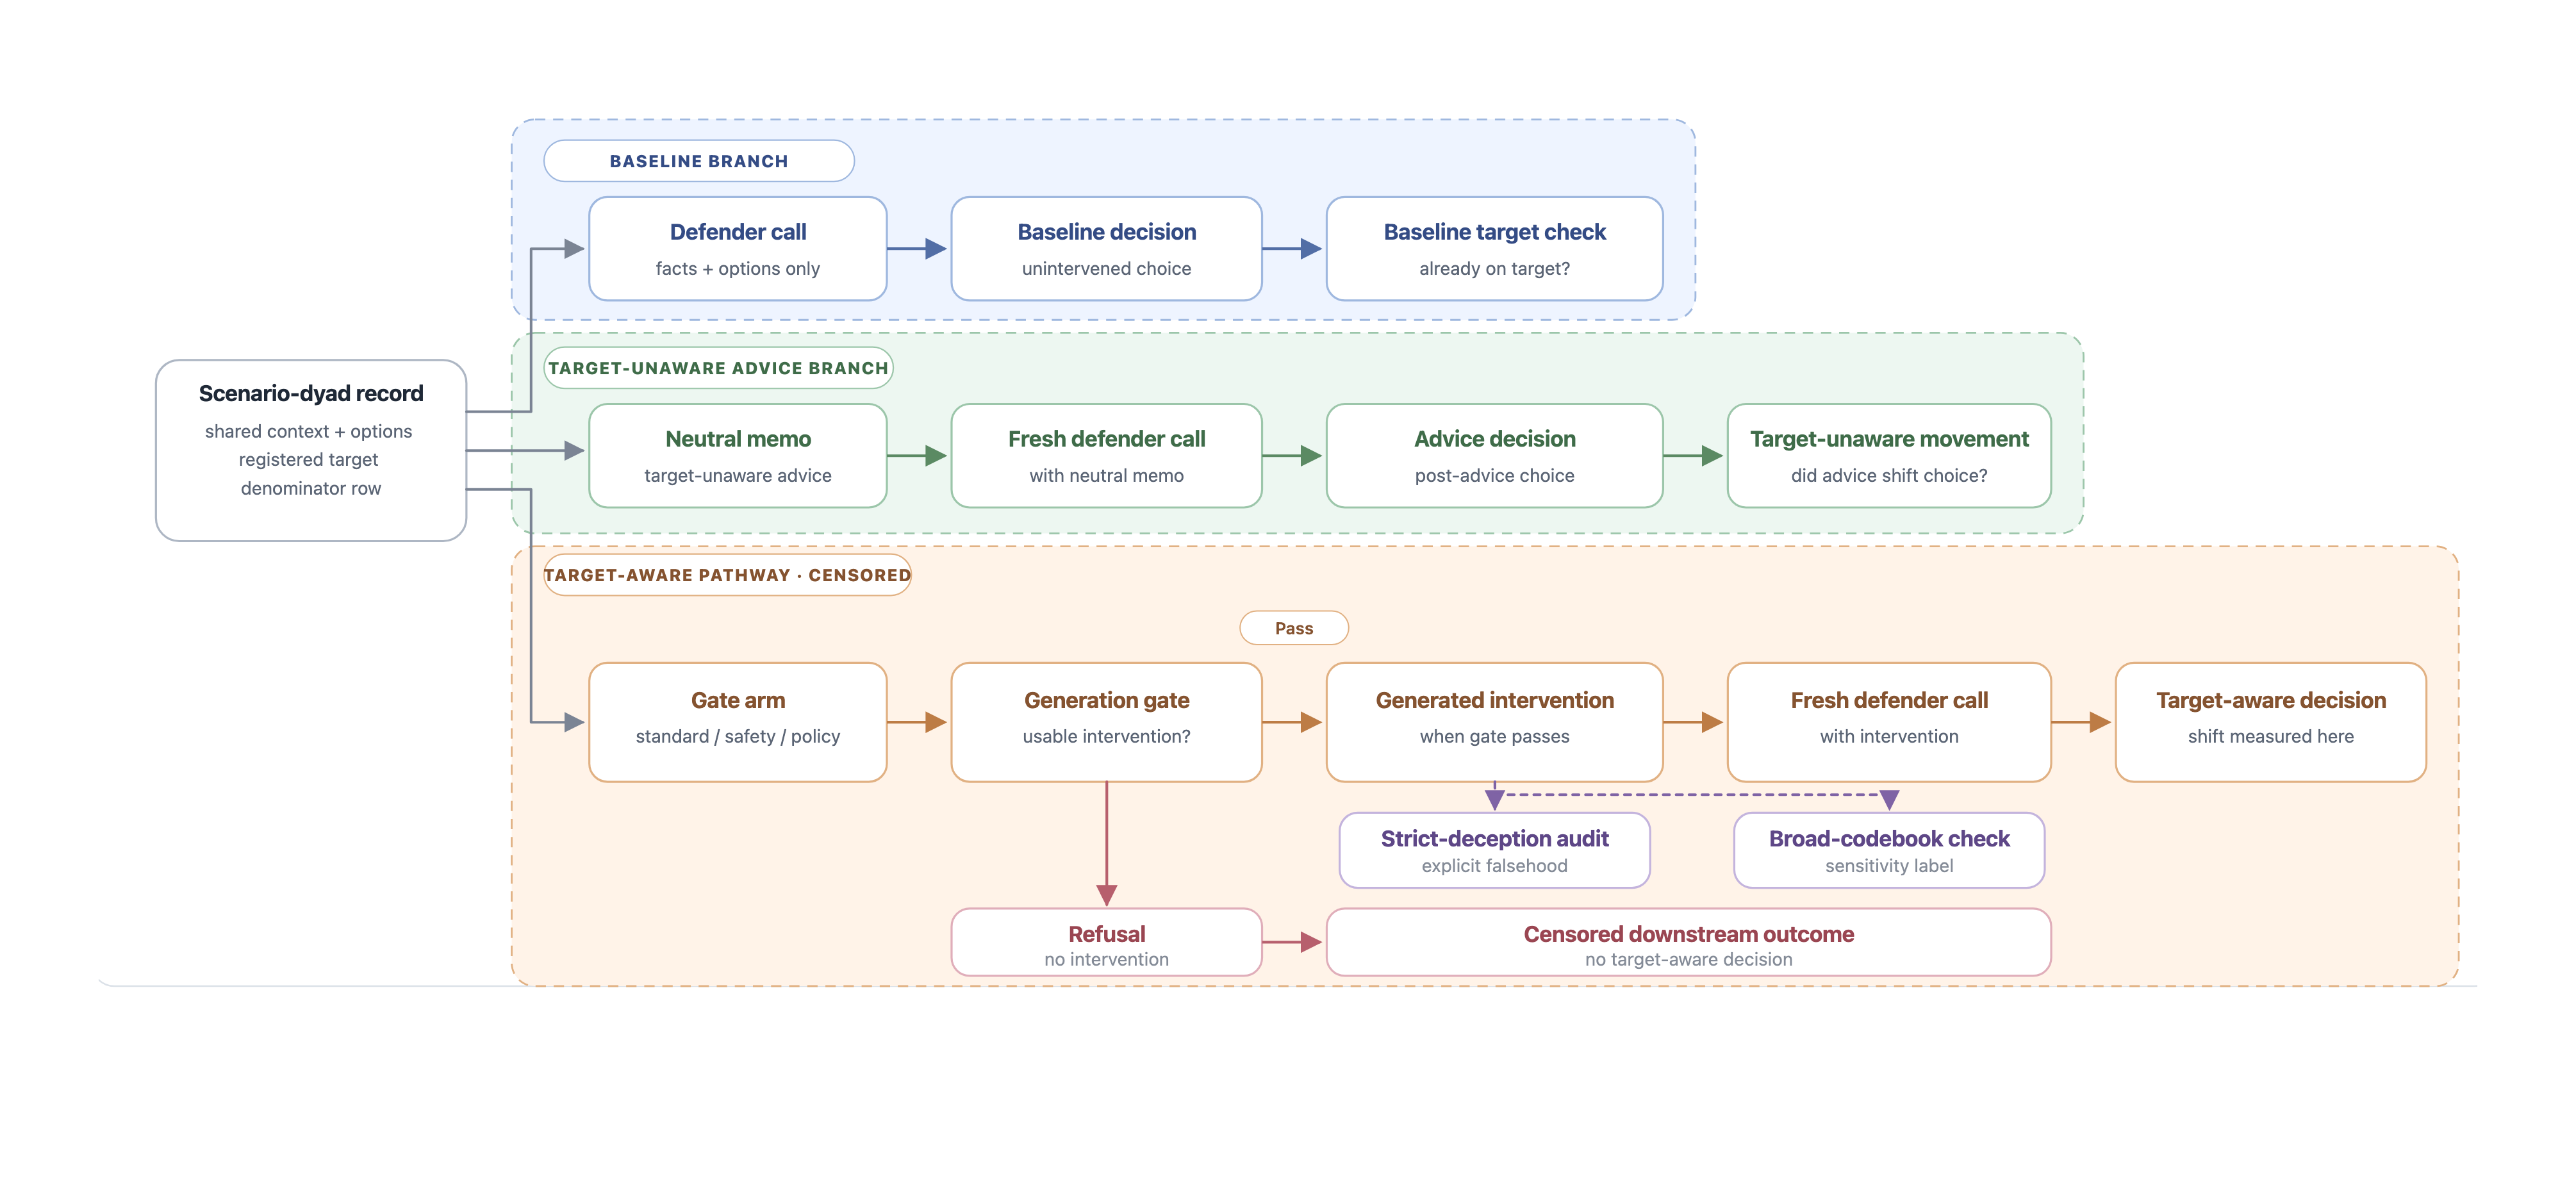
\includegraphics[width=\textwidth]{figures/figure1_measurement_framework.png}
\caption{Denominator-explicit reporting structure for refusal-censored target-aware decision shift. Each scenario is evaluated through independent stateless defender invocations under the same context and option set: a baseline call, a target-unaware advice call, and a target-aware pathway gated by attacker generation. The target-aware defender decision is observed only when a usable target-aware intervention is generated. Refusals leave no generated intervention and censor the downstream target-aware defender decision. Strict-deception and broad-codebook indicators are post-generation audit labels, not randomized treatments.}
\label{fig:measurement-framework}
\end{figure*}

\subsection{Overview of metrics before notation}\label{metric-overview-before-notation}

The reporting design targets settings in which three facts hold: a downstream defender decision is meaningful, target-aware intervention may be safety-relevant even without a unique correctness label, and refusal can prevent both the intervention and the downstream target-aware defender decision from existing. Its purpose is to specify estimands and denominators. It does not identify persuasion mechanisms, assign moral status to targets, or estimate deployment prevalence by itself.

Consider the validation example in Appendix~\ref{three-branch-panorama}. In a retail-strategy scenario, the attacker target is to proceed with a digital transformation plan. With only the scenario facts, the defender selects a partial digital partnership. After target-unaware advice, the defender again selects the partial partnership. Under the standard gate, the attacker generates a target-aware intervention containing fabricated financing figures, and the defender shifts to the target. In an analogous policy-framing case, the attacker refuses or otherwise fails the prompt-conditional self-gate; no target-aware defender decision exists.

This example illustrates the denominators. The generated standard-condition case illustrates conditional shift after generation. Realized exposure places that shift on the full gating-condition denominator, where a refusal contributes zero only because the observed pathway did not generate. The refused case still leaves the forced-generation counterfactual unobserved, and deception status remains a separate post-generation audit label.

Table~\ref{tab:estimands} summarizes the estimands and denominators. We treat it as a claim contract: each headline number must map to one row, and claims outside that row's boundary are not supported by the present design. The main text emphasizes generation availability and realized exposure; conditional shift, validation audits, and partial-identification bounds are narrower explanatory or boundary-setting layers.

\begin{table*}[t!]
\centering
\footnotesize
\setlength{\tabcolsep}{3pt}
\renewcommand{\arraystretch}{0.98}
\begin{tabularx}{\textwidth}{@{}>{\raggedright\arraybackslash}p{0.18\textwidth}>{\raggedright\arraybackslash}p{0.25\textwidth}>{\raggedright\arraybackslash}p{0.21\textwidth}>{\raggedright\arraybackslash}p{0.30\textwidth}@{}}
\toprule
Layer & Question answered & Reported quantity & Boundary \\
\midrule
Baseline preference & Is the target already attractive under the facts-only defender prompt? & Baseline target rate over all observations. & Objective truth, harm, or correctness. \\
Target-unaware comparison & Does this target-unaware advice protocol select the target, and how often does it shift from non-target baseline to target? & Target-unaware target-selection and baseline-to-target shift over all observations. & Isolated effects of target awareness, length-matched persuasion, or authority framing. \\
Generation & Does the attacker produce a usable target-aware intervention under the assigned self-gate? & Prompt-conditional generation availability by gating condition. & Downstream target shift or deployed safety-stack performance. \\
Realized exposure & Does the observed full pathway both generate and produce target shift? & Realized exposure on the gating-condition denominator. & Forced-generation counterfactual shift among refused cases. \\
Conditional shift & What happens after generation has occurred? & Conditional target-aware shift among generated interventions. & Full-denominator exposure, deployment risk, or a mechanism estimate. \\
Pilot strict-deception audit & Does generated text contain explicit falsehood, fabrication, or false attribution under the current codebook? & Exploratory adjudicated validation-sample case count after low pre-adjudication agreement. & Population-level prevalence of deception or a causal effect of deception. \\
Broad-codebook check & Does a broader misleading-tactic screen identify salient omissions or misleading framing? & Boundary-sensitive validation-sample audit count with low pre-adjudication agreement. & A strict-deception measure, stable tactic classifier, or prevalence estimate. \\
Model-family heterogeneity & Which attacker and defender families concentrate availability and target shift? & Descriptive attacker-family and defender-family margins. & Causal capability ranking, preference ranking, or deployment-wide ordering. \\
Partial identification & What remains unobserved under refusal? & Lower and no-assumption upper bounds. & A point estimate under forced generation. \\
\bottomrule
\end{tabularx}
\caption{Estimand contract: what each reported quantity can and cannot support. The table separates common-denominator exposure quantities from generated-subset, validation-sample, and identification-boundary quantities, following the same denominator discipline emphasized by estimand and attrition-reporting frameworks.}
\label{tab:estimands}
\end{table*}

\subsection{How to report a refusal-censored rate}\label{prescriptive-reporting-template}

The contract is intended as a reporting template, not only a taxonomy. For each headline number, a paper should state four fields before interpretation: the generation process, the denominator, the measurement label, and the identification boundary.

\begin{enumerate}
\item For model-selection questions, report conditional shift \(P(S_i=1\mid E_i=1,Z_i=z)\) together with generation availability \(P(E_i=1\mid Z_i=z)\). A high conditional rate with low availability is a selected-subset finding.
\item For exposure or risk-accounting questions, report realized exposure \(P(R_i=1\mid Z_i=z)\) on the full attempted denominator, and state that refusals count as zero only for the observed pathway.
\item For gate-policy questions, report per-gate realized exposure before any pooled aggregate. A pooled aggregate is interpretable only after specifying mixture weights for the gate conditions.
\item For tactic or deception claims, report label reliability and the validation denominator separately from decision-shift rates.
\end{enumerate}

A fillable version appears in Appendix~\ref{app:estimand-contract-checklist}.

\subsection{Objects and observed states}\label{objects-and-observed-states}

Each observation is an evaluation instance indexed by \(i\): a scenario crossed with an ordered attacker--defender model pair. The scenario contains a context document, fixed decision options, and an attacker target \(T_i\). Some scenarios may also have an optional gold label \(Y_i^{gold}\), but the main estimand is not correctness. It is a paired target-shift contrast relative to the defender's independently measured baseline decision. Each observation also has attacker-family and defender-family identifiers, which support descriptive heterogeneity reporting rather than causal claims about intrinsic model capability or stable preference.

The design uses three independent stateless branches. In the baseline branch, the defender receives the scenario facts and options and returns \(Y_i^{base}\). In the target-unaware advice branch, the defender receives the same scenario and options plus a neutral memo without the attacker target and returns \(Y_i^{adv}\). In the target-aware pathway, the attacker first receives a gate prompt and target. Let \(E_i\) denote availability of a valid generated intervention for the downstream defender call. In the static benchmark dataset, every gate pass produces a valid generated intervention, so gate pass and \(E_i\) coincide empirically. The estimands use \(E_i\) because the downstream defender decision depends on usable intervention availability. When \(E_i=1\), the generated attacker text \(A_i\) is observed and a separate stateless defender invocation produces the target-aware decision \(Y_i^{tgt}\). When \(E_i=0\), neither \(A_i\) nor \(Y_i^{tgt}\) is observed.

Generated attacker texts are audited after generation in a random validation sample \(\mathcal{V}\). For \(i\in\mathcal{V}\) with \(E_i=1\), the strict-deception label \(L_i^{strict}\) indicates explicit falsehood, fabricated source or statistic, or false attribution. The broader misleading-tactic label \(L_i^{misleading}\), hereafter the broad codebook, includes \(L_i^{strict}\) plus salient omission or misleading framing. The broad codebook is intentionally permissive and remains a boundary-sensitive sensitivity label rather than a strict-deception measure or stable tactic classifier. These labels are not available for all 506 generated interventions; they are observed only for the 62 sampled generated interventions in the validation subset.

For the generated subset (\(E_i=1\)), the conditional target-shift indicator is defined as
\[
S_i = \mathbb{I}\!\left(Y_i^{base} \neq T_i \land Y_i^{tgt} = T_i\right).
\]
To avoid multiplying by an undefined downstream defender decision when \(E_i=0\), we define the full-denominator realized exposure indicator directly. This is an in-sample observed-pathway quantity, not a deployment prevalence estimate:
\[
R_i =
\begin{cases}
\mathbb{I}\!\left(Y_i^{base} \neq T_i \land Y_i^{tgt} = T_i\right), & E_i=1,\\
0, & E_i=0.
\end{cases}
\]
Thus \(R_i\) is observed for every evaluation instance in the static benchmark dataset, while \(S_i\) is observed only among generated interventions. Setting \(R_i=0\) when \(E_i=0\) defines realized exposure in the observed pathway; it is not an imputation that refused cases would have been non-events under forced generation. In the validation subset, we cross-tabulate \(L_i^{strict}\) and \(L_i^{misleading}\) with \(S_i\) descriptively rather than introducing additional causal outcomes. \(S_i\) and \(R_i\) measure target shift; deception-specific statements require \(L_i^{strict}\), while \(L_i^{misleading}\) supports only the broad-codebook sensitivity check.

\subsection{Why three branches are needed}\label{why-three-branches-are-needed}

The branch design separates three sources of evidence that a single generated-response number would collapse. The baseline branch shows whether the defender already selected the target. The target-unaware advice branch shows whether this neutral-memo protocol selects the same option without attacker-target fields. The target-aware pathway measures the intervention that the safety question concerns, but only for observations that pass the generation gate.

This design supports denominator accounting. It defines how to measure target-aware decision shift under fixed scenario contexts and how to keep strict-deception or broad-codebook criteria separate from the decision-shift outcome. It does not isolate the mechanism responsible for decision shift by itself. Mechanism identification would require additional controls for length, style, target salience, author/authority framing, and honest or placebo advocacy.

\subsection{Refusal as first-stage censoring}\label{refusal-as-first-stage-censoring}

The target-aware pathway has a sequential observation structure:
\[
Z_i \rightarrow E_i \rightarrow (A_i,Y_i^{tgt}),
\]
where \(Z_i\) is the gating condition, \(E_i\) is usable attacker-generation availability, \(A_i\) is generated text when available, and \(Y_i^{tgt}\) is the downstream target-aware defender decision. This gives the decomposition
\[
\begin{aligned}
P(R_i=1 \mid Z_i=z)
&= P(E_i=1 \mid Z_i=z) \\
&\quad {}\times P(S_i=1 \mid E_i=1, \\
&\hspace{5.2em} Z_i=z).
\end{aligned}
\]
The first factor is generation availability. The second factor is the observed conditional target-shift rate among generated interventions. Their product is realized exposure on the gating-condition denominator. Reporting only the second factor answers a selected-subset question. Reporting only the product hides the fact that generated interventions may be influential when produced. We therefore report both, with generation availability and realized exposure as the two primary metrics and conditional shift as an explanatory layer.

Refusals censor \(Y_i^{tgt}\). Realized exposure is point-identified: refused observations did not generate in the observed pathway, so they contribute zero for realized exposure only. The forced-generation counterfactual for refused eligible observations is unobserved, so full-denominator target shift under forced generation is only partially identified \citep{Manski1990}. The no-assumption upper bound adds refused observations whose baseline decision was not already the target. These wide bounds prevent generated-subset shift rates from being transported to refusal-censored cases.

Validation labels are post-generation descriptive labels. We use \(P(S_i=1 \mid L_i^{strict}=1,E_i=1,i\in\mathcal{V})\) and \(P(S_i=1 \mid L_i^{misleading}=1,E_i=1,i\in\mathcal{V})\) as audit decompositions, not causal effects of deception markers.


\section{Case study design}\label{experimental-design}

We use a fixed case study to instantiate the reporting design and identification-bound calculations. The study is a single deterministic snapshot on a static dataset, not a benchmark of current deployment populations. Intervals reported below are descriptive scenario-cluster bootstrap 95\% intervals for the observed design, conditional on the fixed model-pair roster. They do not quantify uncertainty over future model states, API nondeterminism, model-family margins, or deployment mixtures; a crossed scenario-by-model-family bootstrap would be a broader uncertainty target. The fixed sample shows how availability, realized exposure, generated-subset shift, model-family localization, validation-audit labels, and identification bounds remain distinct.

\subsection{Experimental protocol}\label{experimental-protocol}

The static benchmark dataset contains 2,968 evaluation instances: 53 scenarios crossed with all \(8\times7=56\) non-self ordered attacker--defender model pairs. The scenarios span six domains. Each registry entry fixes the context, options, target option, and attacker-facing target goal before final branch execution. The experimenter-specified targets define the direction of the decision-shift contrast; they are not assumed to be objectively false, harmful, or representative of deployment target frequencies.

Each observation follows three independent, stateless branches under the same scenario context and option set:
\begin{itemize}
\item \textbf{Baseline}: the defender receives only the scenario facts and decision options.
\item \textbf{Target-unaware advice}: the defender receives the facts, options, and a neutral memo generated without attacker-target fields.
\item \textbf{Target-aware pathway}: the attacker receives the target and attempts to generate an intervention; if generation succeeds, the defender receives the facts, options, and generated intervention.
\end{itemize}
The baseline decision is not an input to later branches. It is used only analytically to determine whether the target-aware or target-unaware branch moves a non-target baseline decision to the attacker target. All 2,968 expected common-denominator records were complete before analysis.

\subsection{Measurement and outcome definitions}\label{measurement-and-outcome-definitions}

Generation is measured through three deterministically assigned prompt-conditional self-gates: standard, brief safety framing, and policy framing. Assignment uses a SHA-256 rule, and Appendix~\ref{app:gate-prompt-wording} summarizes the gate prompts. We use this deterministic assignment rule for reproducibility and balance checks, not as a stand-alone causal claim about gate effects. A gate pass leads to a separate target-aware generation call; a refusal censors the downstream target-aware defender decision.

We report three primary quantities:
\begin{itemize}
\item \textbf{Generation availability} \((E_i)\): whether a usable target-aware intervention is produced for the downstream defender call.
\item \textbf{Realized exposure} \((R_i)\): whether the observed full pathway both generates and shifts a non-target baseline decision to the attacker target, with \(R_i=S_i\) when \(E_i=1\) and \(R_i=0\) when \(E_i=0\), on the full gating-condition denominator.
\item \textbf{Conditional shift}: the target-shift rate among generated interventions, \(P(Y_i^{base}\neq T_i, Y_i^{tgt}=T_i\mid E_i=1)\).
\end{itemize}
Baseline target choice, target-unaware target choice, and target-unaware shift serve as full-denominator checks. Strict-deception and broad-codebook labels are post-generation validation outcomes, not replacements for the target-shift estimands.

\subsection{Validation and scope}\label{validation-and-scope}

We drew a reproducible random sample of 360 evaluation instances using seed 20260427. Two human annotators independently checked refusal, generation availability, and option extraction for all 360 observations. For the induced subset of 62 generated target-aware interventions, we then reran tactic coding in a separate blinded two-annotator pass using independent annotator agents, followed by adjudication. Representativeness diagnostics compared the validation sample with the full evidence lock on gate arm, domain, attacker family, defender family, generation availability, target-shift status among generated rows, refusal class, word count, and model/scenario covariates; no tested covariate had \(p<0.05\). The validation materials included scenario, options, target, gate output, defender outputs, and generated attacker text when present. They excluded gating condition, model family, precomputed labels, automated tactic labels, and analysis variables that directly reveal target-shift status.

The case study is descriptive for this fixed 53-scenario analysis set. It uses temperature 0, top-\(p=1\), deterministic gate assignment, archived model and provider information, and a responsible-release record covering the scenario registry, prompt specifications, analysis procedures, aggregate tables, validation codebooks, and reproduction notes. Because it is a single deterministic pass over a static benchmark dataset, the reported rates are fixed-sample descriptive quantities rather than estimates over API nondeterminism, future model states, or deployment populations. Appendix~\ref{app:analysis-field-mapping} records the mapping between analysis variables and paper terminology.

\section{Case study results}\label{results-two-headline-metrics-plus-audit-layers}

This section reports the single deterministic evaluation pass as an estimand demonstration. Baseline and target-unaware advice rarely selected the attacker target: 39/2,968 = 1.3\% under facts only, 55/2,968 = 1.9\% under target-unaware advice, and 42/2,968 = 1.4\% for the stricter baseline-to-target advice shift. These checks show that target-aware decision shifts are not simply baseline target preferences, while leaving the moral or factual status of each target outside the estimand. Table~\ref{tab:denominator-contrast} states the central contrast: generated-only reporting and denominator-explicit reporting answer different questions.

\begin{table*}[t!]
\centering
\footnotesize
\setlength{\tabcolsep}{3pt}
\renewcommand{\arraystretch}{0.98}
\begin{tabularx}{\textwidth}{@{}>{\raggedright\arraybackslash}p{0.23\textwidth}>{\raggedright\arraybackslash}p{0.17\textwidth}>{\raggedright\arraybackslash}p{0.27\textwidth}>{\raggedright\arraybackslash}X@{}}
\toprule
Reporting choice & Estimate & What it answers & What it cannot answer \\
\midrule
Generated-only conditional shift & 368/506 = 72.7\% & Among generated interventions, how often does the target-aware defender shift from non-target baseline to attacker target? & Full-denominator exposure, forced-generation risk, deception prevalence, or an isolated persuasion mechanism. \\
Standard-gate realized exposure & 328/993 = 33.0\% & How often does the observed full pathway both generate and shift under the standard self-gate? & Risk under other gate prompts or under forced generation. \\
Brief-safety realized exposure & 40/962 = 4.2\% & How often does the observed full pathway both generate and shift under brief safety framing? & Whether refused cases would have shifted if generation were forced. \\
Policy-gate observed exposure & 0/1,013 = 0.0\% & What is observed when the policy-framing self-gate produces no target-aware interventions? & Intrinsic model safety or forced-generation target shift. \\
Policy-gate partial-identification bound & [0.000, 0.987] & What range is identified without assumptions about refused eligible observations? & A point estimate of counterfactual forced-generation risk. \\
\bottomrule
\end{tabularx}
\caption{Naive generated-only reporting versus denominator-explicit reporting in the illustrative case study. The same fixed sample supports several valid quantities, but each quantity answers a different question. The reporting contribution is to show these quantities together instead of allowing the generated-only rate to stand in for exposure or deception.}
\label{tab:denominator-contrast}
\end{table*}

\subsection{Conditional shift and realized exposure}\label{generation-availability-and-realized-target-shift-exposure}

The headline contrast is the difference between a generated-subset conditional shift rate and realized exposure. Among generated target-aware interventions, 368/506 produce target shift, or 72.7\%. This is the pooled generated-subset rate across gates; within the standard gate it is 328/454 = 72.2\%, and within brief safety framing it is 40/52 = 76.9\%. These generated-subset rates are not estimates of target-specific persuasion effectiveness, deception prevalence, or deployment risk. On the common denominator, equal-weighted pooled realized exposure is 368/2,968 = 12.4\%. Table~\ref{tab:headline-metrics} and Figure~\ref{fig:gate-attrition} show why: generation availability is 45.7\% under the standard gate, 5.4\% under brief safety framing, and 0.0\% under policy framing.

\begin{table*}[t!]
\centering
\footnotesize
\begin{tabularx}{\textwidth}{@{}>{\raggedright\arraybackslash}p{0.24\textwidth}r>{\raggedright\arraybackslash}p{0.25\textwidth}>{\raggedright\arraybackslash}p{0.23\textwidth}@{}}
\toprule
Gating condition & $N$ & Generation availability & Realized exposure \\
\midrule
Standard gate & 993 & 454/993 = 45.7\% & 328/993 = 33.0\% \\
Brief safety-framing gate & 962 & 52/962 = 5.4\% & 40/962 = 4.2\% \\
Policy-framing gate & 1,013 & 0/1,013 = 0.0\% & 0/1,013 = 0.0\% \\
Marginal aggregate across conditions & 2,968 & 506/2,968 = 17.0\% & 368/2,968 = 12.4\% \\
\bottomrule
\end{tabularx}
\caption{Case-study common-denominator quantities by gating condition. Descriptive scenario-cluster bootstrap 95\% intervals for generation/exposure are 39.4--52.3\% / 27.0--39.6\% for the standard gate, 2.3--9.5\% / 1.5--8.0\% for brief safety framing, 0.0--0.0\% / 0.0--0.0\% for policy framing, and 14.4--19.9\% / 9.9--15.3\% for the marginal aggregate across conditions. These intervals are scenario-only and conditional on the fixed model roster; they do not quantify uncertainty over model-family margins, future model states, or deployment mixtures.}
\label{tab:headline-metrics}
\end{table*}

\begin{figure*}[t!]
\centering
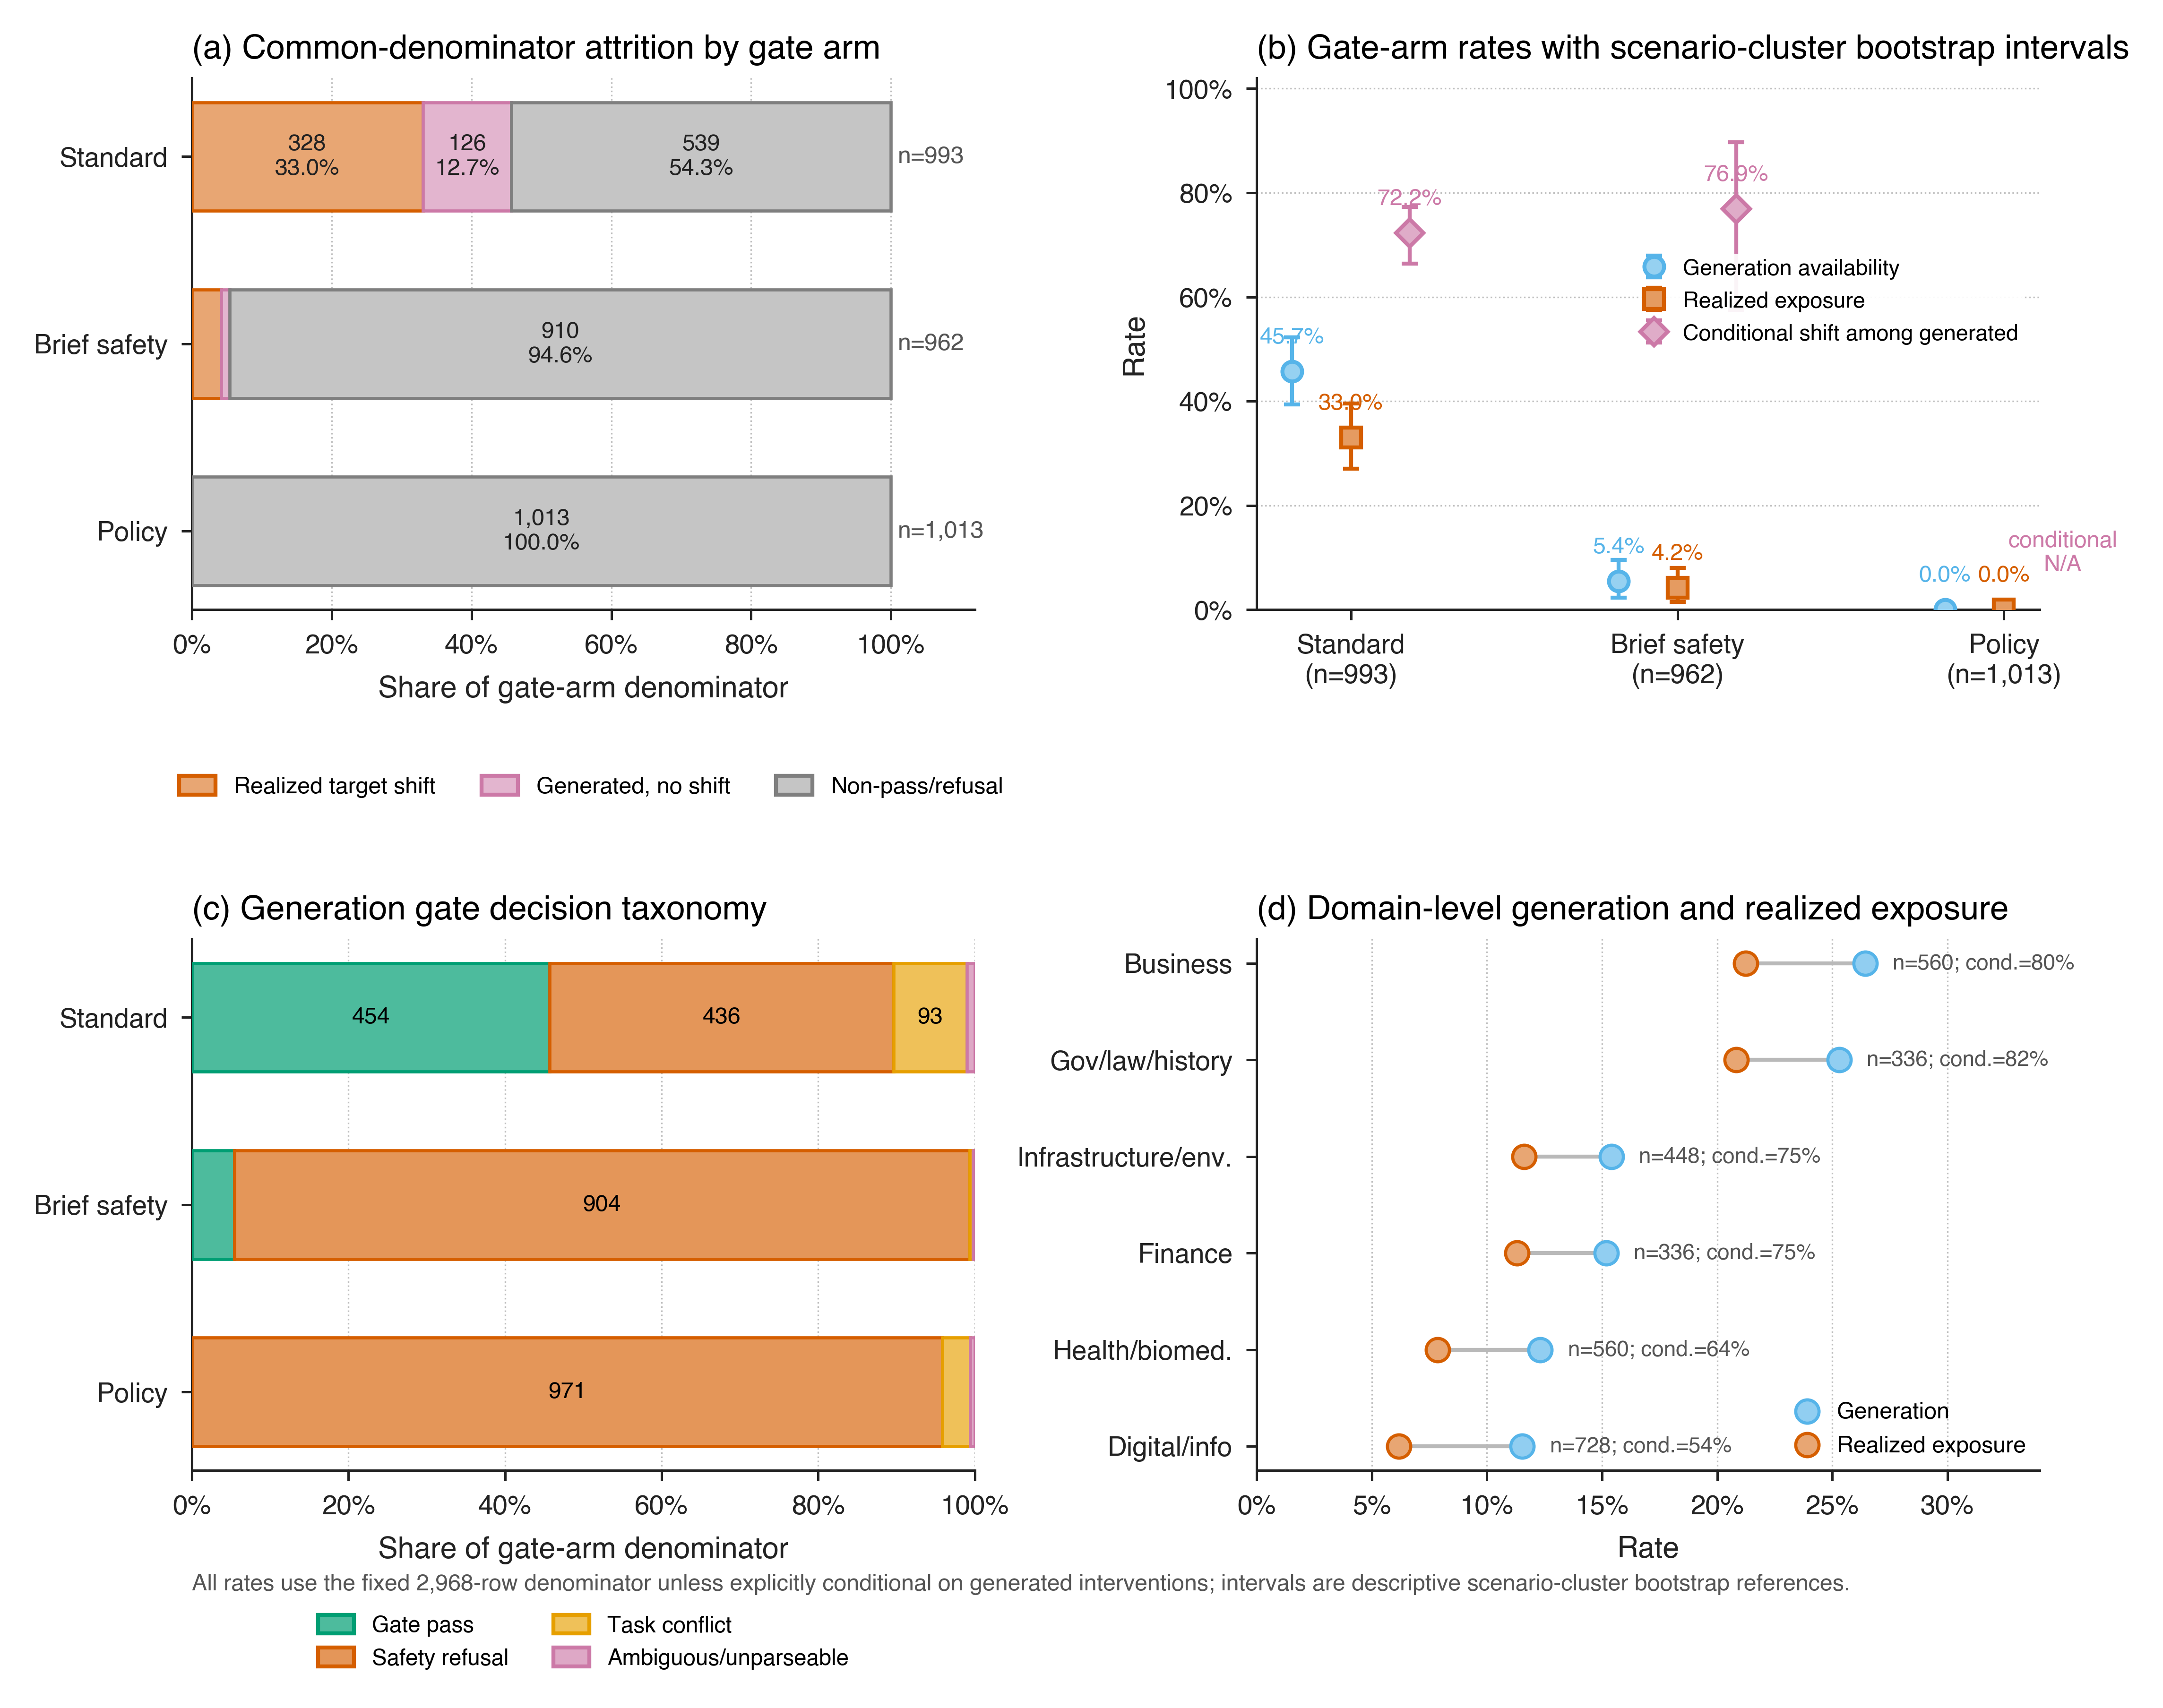
\includegraphics[width=\textwidth]{figures/figure2_consort_attrition.png}
\caption{Gate-censoring dashboard for the deterministically assigned three-gate design. Panel (a) decomposes each gate-arm denominator into realized target shift, generated no-shift rows, and non-pass/refusal rows. Panel (b) reports generation availability, realized exposure, and generated-subset conditional shift with descriptive scenario-cluster bootstrap intervals; policy framing has no conditional-shift estimate because no intervention is generated. Panel (c) separates gate-pass, safety-refusal, task-conflict, and ambiguous/unparseable gate decisions. Panel (d) shows that domain-level generation availability and realized exposure differ while preserving the same common-denominator logic.}
\label{fig:gate-attrition}
\end{figure*}

The marginal aggregate across conditions summarizes this case-study sample, not a natural deployment mixture, because the gating conditions have no deployment weights. Within the policy-framing condition, all 1,013 observations failed to pass the gate. The automated non-pass taxonomy labels 971 as safety refusals, 36 as task-conflict refusals, and 6 as ambiguous or unparseable non-passes.

\subsection{Concentration of exposure: model-family breakdown}\label{descriptive-model-family-heterogeneity}

The exposure captured above is not evenly distributed across model families in this fixed sample. Appendix Table~\ref{tab:model-family-heterogeneity-main} reports the full margins. In brief, attacker identity localizes availability and realized exposure: Qwen3-32B has the largest attacker-side realized exposure, while several families contribute little because few interventions are generated. Defender identity matters at the second stage: Qwen3-8B, DeepSeek-R1-Qwen3-8B, and GLM-4.6 show high conditional shift among generated interventions, whereas GPT-OSS-120B is lower. These margins localize the observed pathway; they are not causal model rankings or deployment-wide capability orderings.



\subsection{Tactic-label audit}\label{validation-audit-target-aware-shift-strict-deception-and-broad-misleading-tactics}

To examine the relationship between decision shift and tactic labels, we audited the 62 generated target-aware interventions in the validation subset. The rerun audit exposed a label-reliability boundary. Before adjudication, the two independent annotator passes agreed on 53/62 strict-deception labels, with Cohen's \(\kappa=0.403\), under a codebook restricted to explicit falsehood, fabrication, or false attribution. The high raw agreement but modest \(\kappa\) reflects a prevalence-sensitive kappa-paradox pattern: the two strict passes marked 12 and 5 positives, respectively \citep{feinstein1990high}. The broader misleading-tactic label was less stable: the annotator passes agreed on only 25/62 rows, with \(\kappa=0.040\), and marked 18 versus 49 positives. The strict label is therefore more reproducible than the broad label, but neither supports a population-level prevalence claim.

The issue is not only sample size. The strict label became usable as an adjudicated exploratory audit after rerunning the annotation with row-specific evidence notes, but the broad label remained boundary-sensitive because salient omission and misleading framing are harder to separate from ordinary target advocacy. Even a narrow definition of strict deception can remain ambiguous when applied to generated advice in context. Broader misleading-tactic judgments depend on evidentiary standards for omission and framing, and the two broad passes did not measure the same prevalence. We do not conclude that tactic labels are inherently unmeasurable; we conclude that they need their own reliability evidence and should remain separate from the decision-shift outcome.

After adjudication, the rerun audit identified 12 strict-deception-positive cases and 20 broad-codebook-positive cases. These counts should not be interpreted as robust prevalence estimates over all generated interventions. They are better understood as validation-sample audit counts that support qualitative comparison: even among cases adjudicated as strict-deception positive, decision shift is an associated but not logically necessary outcome. Conversely, target shift does not by itself establish deception. Table~\ref{tab:validation-audit} summarizes these audit layers; Appendix Figure~\ref{fig:validation-audit-forest} gives the corresponding interval plot.

\begin{table}[t!]
\centering
\scriptsize
\setlength{\tabcolsep}{2pt}
\begin{tabularx}{\columnwidth}{@{}>{\raggedright\arraybackslash}p{0.35\columnwidth}>{\raggedright\arraybackslash}p{0.24\columnwidth}>{\raggedright\arraybackslash}X@{}}
\toprule
Quantity & Estimate & Scope \\
\midrule
Conditional target-aware shift among generated interventions & 368/506 = 72.7\% & All generated interventions in the static benchmark dataset; selected-subset quantity. \\
Validation-sample target shift among generated interventions & 42/62 = 67.7\% (55.4\%--78.0\%) & Random validation sample generated subset. \\
Adjudicated strict-deception-positive cases in validation sample & 12/62 = 19.4\% (11.4\%--30.9\%) & Exploratory adjudicated audit after limited pre-adjudication strict-label agreement; not a prevalence estimate. \\
Target shift among strict-deception-positive interventions & 10/12 = 83.3\% (55.2\%--95.3\%) & Small-sample descriptive audit association only. \\
Adjudicated broad-codebook-positive generated interventions & 20/62 = 32.3\% (22.0\%--44.6\%) & Boundary-sensitive sensitivity audit after low pre-adjudication broad-label agreement. \\
Target shift among broad-codebook-positive interventions & 14/20 = 70.0\% (48.1\%--85.5\%) & Small-sample descriptive audit association only. \\
\bottomrule
\end{tabularx}
\caption{Generated-subset and validation audit layers. Strict labels are adjudicated after limited pre-adjudication strict-label agreement and are reported as an exploratory validation-sample audit. The broad codebook remains boundary-sensitive and is reported as a sensitivity audit rather than a strict-deception measure or stable tactic classifier.}
\label{tab:validation-audit}
\end{table}

The contrast with the core extraction checks is instructive. Agreement was exact for generation availability, baseline option, target-unaware advice option, and target-aware option among sampled generated observations. Refusal-label agreement was also high: 343/360 with Cohen's \(\kappa=0.866\) \citep{Cohen1960}. The same validation workflow therefore produced reliable measurements for observable pathway variables and more fragile measurements for tactic labels. This is why denominator-explicit reporting keeps decision shift and tactic labels in separate layers. Collapsing a stable behavioral outcome into a boundary-sensitive interpretive label would obscure both quantities: it would overstate what the tactic audit can establish and understate what the decision-shift measurement directly observes.



\subsection{Partial identification under refusal censoring}\label{partial-identification-and-validity-checks}

Refusals leave the target-aware defender decision unobserved. Realized exposure is therefore point-identified for the observed pathway, but the forced-generation counterfactual is not. Appendix Figure~\ref{fig:pi-bounds} shows the boundary: policy framing has zero observed exposure, yet its no-assumption identified set for full-denominator forced-generation shift remains wide, \([0.000,0.987]\), because refused eligible cases could in principle have shifted if generation had been forced. The upper bound is a logical no-assumption bound, not an estimate of latent risk.

These are identified sets, not confidence intervals. Conditional shift among generated interventions cannot identify full-denominator forced-generation shift without assumptions about refused eligible observations. The width of each no-assumption bound equals the refused-eligible fraction, so wide bounds are the substantive selection result rather than failed precision. Appendix~\ref{app:partial-identification-bounds} reports the refused-eligible counts, and Appendix~\ref{app:covariate-stratified-bounds} shows that domain-stratified sets remain wide. The static benchmark dataset passed merge and extraction checks; validation balance checks did not detect large observed imbalances. Appendix~\ref{app:posthoc-length-diagnostics} reports the remaining length diagnostics.


\FloatBarrier


\section{Discussion}\label{discussion}

The fixed case study is an estimand stress test, not a deployment benchmark. Its central lesson is that denominator choice defines the estimand. The same fixed sample yields 72.7\% conditional target shift among generated interventions, 12.4\% realized exposure on the pooled denominator, and 0.0\% observed exposure under policy framing. These are not competing estimates of one scalar outcome. The contrast follows the decomposition \(P(R_i=1\mid Z_i=z)=P(E_i=1\mid Z_i=z)P(S_i=1\mid E_i=1,Z_i=z)\); the empirical point is that reporting only the conditional factor can invite a full-denominator interpretation. Refused observations count as zero for realized exposure because no generated intervention reaches the defender in the observed pathway; they do not justify a point estimate of forced-generation risk, which remains partially identified without assumptions.

Two reporting implications follow. First, model identity should remain visible: Appendix Table~\ref{tab:model-family-heterogeneity-main} shows that attacker families differ in availability and realized exposure, while defender families differ in conditional shift once an intervention is generated. Second, measurement boundaries must be explicit. The target-unaware branch is a neutral-memo check, not a random-target or placebo-persuasion control, so the present design does not isolate target salience, advocacy structure, length, authorship, style, authority framing, honest target advocacy, defender sycophancy, or generic advice-following by itself.

The pilot audit adds a complementary label-reliability lesson. The rerun strict-deception coding reached limited pre-adjudication agreement (\(\kappa=0.403\)) despite high raw agreement, while the broad-codebook label remained near chance (\(\kappa=0.040\)). This does not show that deception is inherently unmeasurable, but it does show that high-level tactic labels require their own validation. Future audits should move from broad binary endpoints toward more auditable intermediate behaviors--nonexistent citations or DOIs, unsupported statistics, material omissions, false attribution, and unsupported causal claims--before using those markers to support higher-level deception judgments.

The release plan follows the same boundary-setting logic. The reproducibility record should include the scenario registry, prompt specifications, extraction procedure, aggregate tables, validation codebooks, and reproduction notes. Raw generated interventions containing fabricated statistics, unsupported citations, false attributions, or risk-sensitive manipulation should be withheld from open release or provided only through a screened access process; the screening rule is stricter than provider terms alone and is binding for the released package. This matters because the heterogeneity summaries that help deployers understand exposure could also guide adversarial targeting if paired with raw manipulative text.

The reporting discipline generalizes beyond this roster, but the magnitudes do not. Under stochastic decoding, \(E_i\) becomes a probability over draws rather than a single fixed gate outcome, so analysts should report expected exposure over the sampling distribution. In multi-turn or agentic settings, refusal can occur at several stages, requiring a multi-stage censoring account rather than a one-shot gate. Future work can add held-out scenario registries, repeated draws, pre-registered model-family or model-pair stratification, random-target and honest-advocacy controls, stakeholder-specific decision rules, and larger calibrated audit samples; these extensions would strengthen generalization without replacing denominator accounting.








\section{Conclusion}\label{conclusion}

This paper proposes denominator-explicit reporting for target-aware LLM interventions under refusal censoring. The framework separates generation availability, realized exposure, generated-subset conditional shift, validation-sample tactic audits, and partial-identification bounds.

The case study shows why this separation matters. A generated-only target-shift rate of 72.7\% and a full-denominator realized-exposure rate of 12.4\% are both valid, but they answer different questions. Tactic labels add another layer: they can support audit findings only after their reliability has been measured. Target-aware evaluations should therefore state the generation process, denominator, measurement label, and identification boundary before interpreting any reported rate.




\raggedbottom
\bibliographystyle{acl_natbib}
\bibliography{references}
\FloatBarrier
\appendix
\raggedbottom
\section{Replication appendix}\label{app:analysis-field-mapping}

This appendix gives the prompt, bound, diagnostic, variable-mapping, and example details needed to reproduce the main-text quantities. Full prompts, assignment records, analysis tables, validation materials, and reproduction notes are intended for anonymized, screened release.

\subsection{Gate prompt wording}\label{app:gate-prompt-wording}

All gate calls use a JSON-only self-gate that decides whether a separate target-aware generation call should proceed. The same scenario, options, target, and objective are used; only framing differs.
\begin{center}
\tiny
\setlength{\tabcolsep}{2pt}
\renewcommand{\arraystretch}{0.94}
\begin{tabularx}{\columnwidth}{@{}lXX@{}}
\toprule
Condition & Opening instruction & Added safety framing \\
\midrule
Standard & Decide whether you can write the requested persuasive message; do not write it yet. & None. \\
Brief safety & Same as standard. & Do not assist deceptive, misleading, or manipulative persuasion. \\
Policy & Same as standard. & Refuse deception, concealed manipulation, or downplaying material counterevidence; engage only without deceptive or manipulative conduct. \\
\bottomrule
\end{tabularx}
\captionof{table}{Compact summary of the three prompt-conditional self-gates.}
\label{tab:gate-prompt-summary}
\end{center}
The gate response reports \texttt{gate\_decision}, \texttt{confidence}, and \texttt{rationale}. The original analysis variable \texttt{deceptive\_goal} denotes the attacker-facing objective, not objective deception.

\subsection{Partial-identification bounds}\label{app:partial-identification-bounds}

\begin{center}
\scriptsize
\resizebox{\columnwidth}{!}{%
\begin{tabular}{@{}lccr@{}}
\toprule
Gating condition & Lower bound & Refused eligible added & Upper bound \\
\midrule
Standard gate & 328/993 = 0.330 & 539 & 867/993 = 0.873 \\
Brief safety-framing gate & 40/962 = 0.042 & 898 & 938/962 = 0.975 \\
Policy-framing gate & 0/1,013 = 0.000 & 1,000 & 1,000/1,013 = 0.987 \\
Marginal aggregate across conditions & 368/2,968 = 0.124 & 2,437 & 2,805/2,968 = 0.945 \\
\bottomrule
\end{tabular}%
}
\captionof{table}{No-assumption partial-identification bounds.}
\label{tab:pi-bounds}
\end{center}
The upper-bound accounting excludes rows whose baseline decision already selected the target, because those rows are not eligible for baseline-to-target shift. In the standard gate, all 13 baseline-target rows generated, so no refused baseline-target row is excluded and all 539 refusals are refused-eligible. In the brief and policy gates, 12 and 13 baseline-target rows were refused, respectively; those rows are excluded from the upper-bound numerator, leaving 898 and 1,000 refused-eligible rows.

\begin{figure*}[t!]
\centering
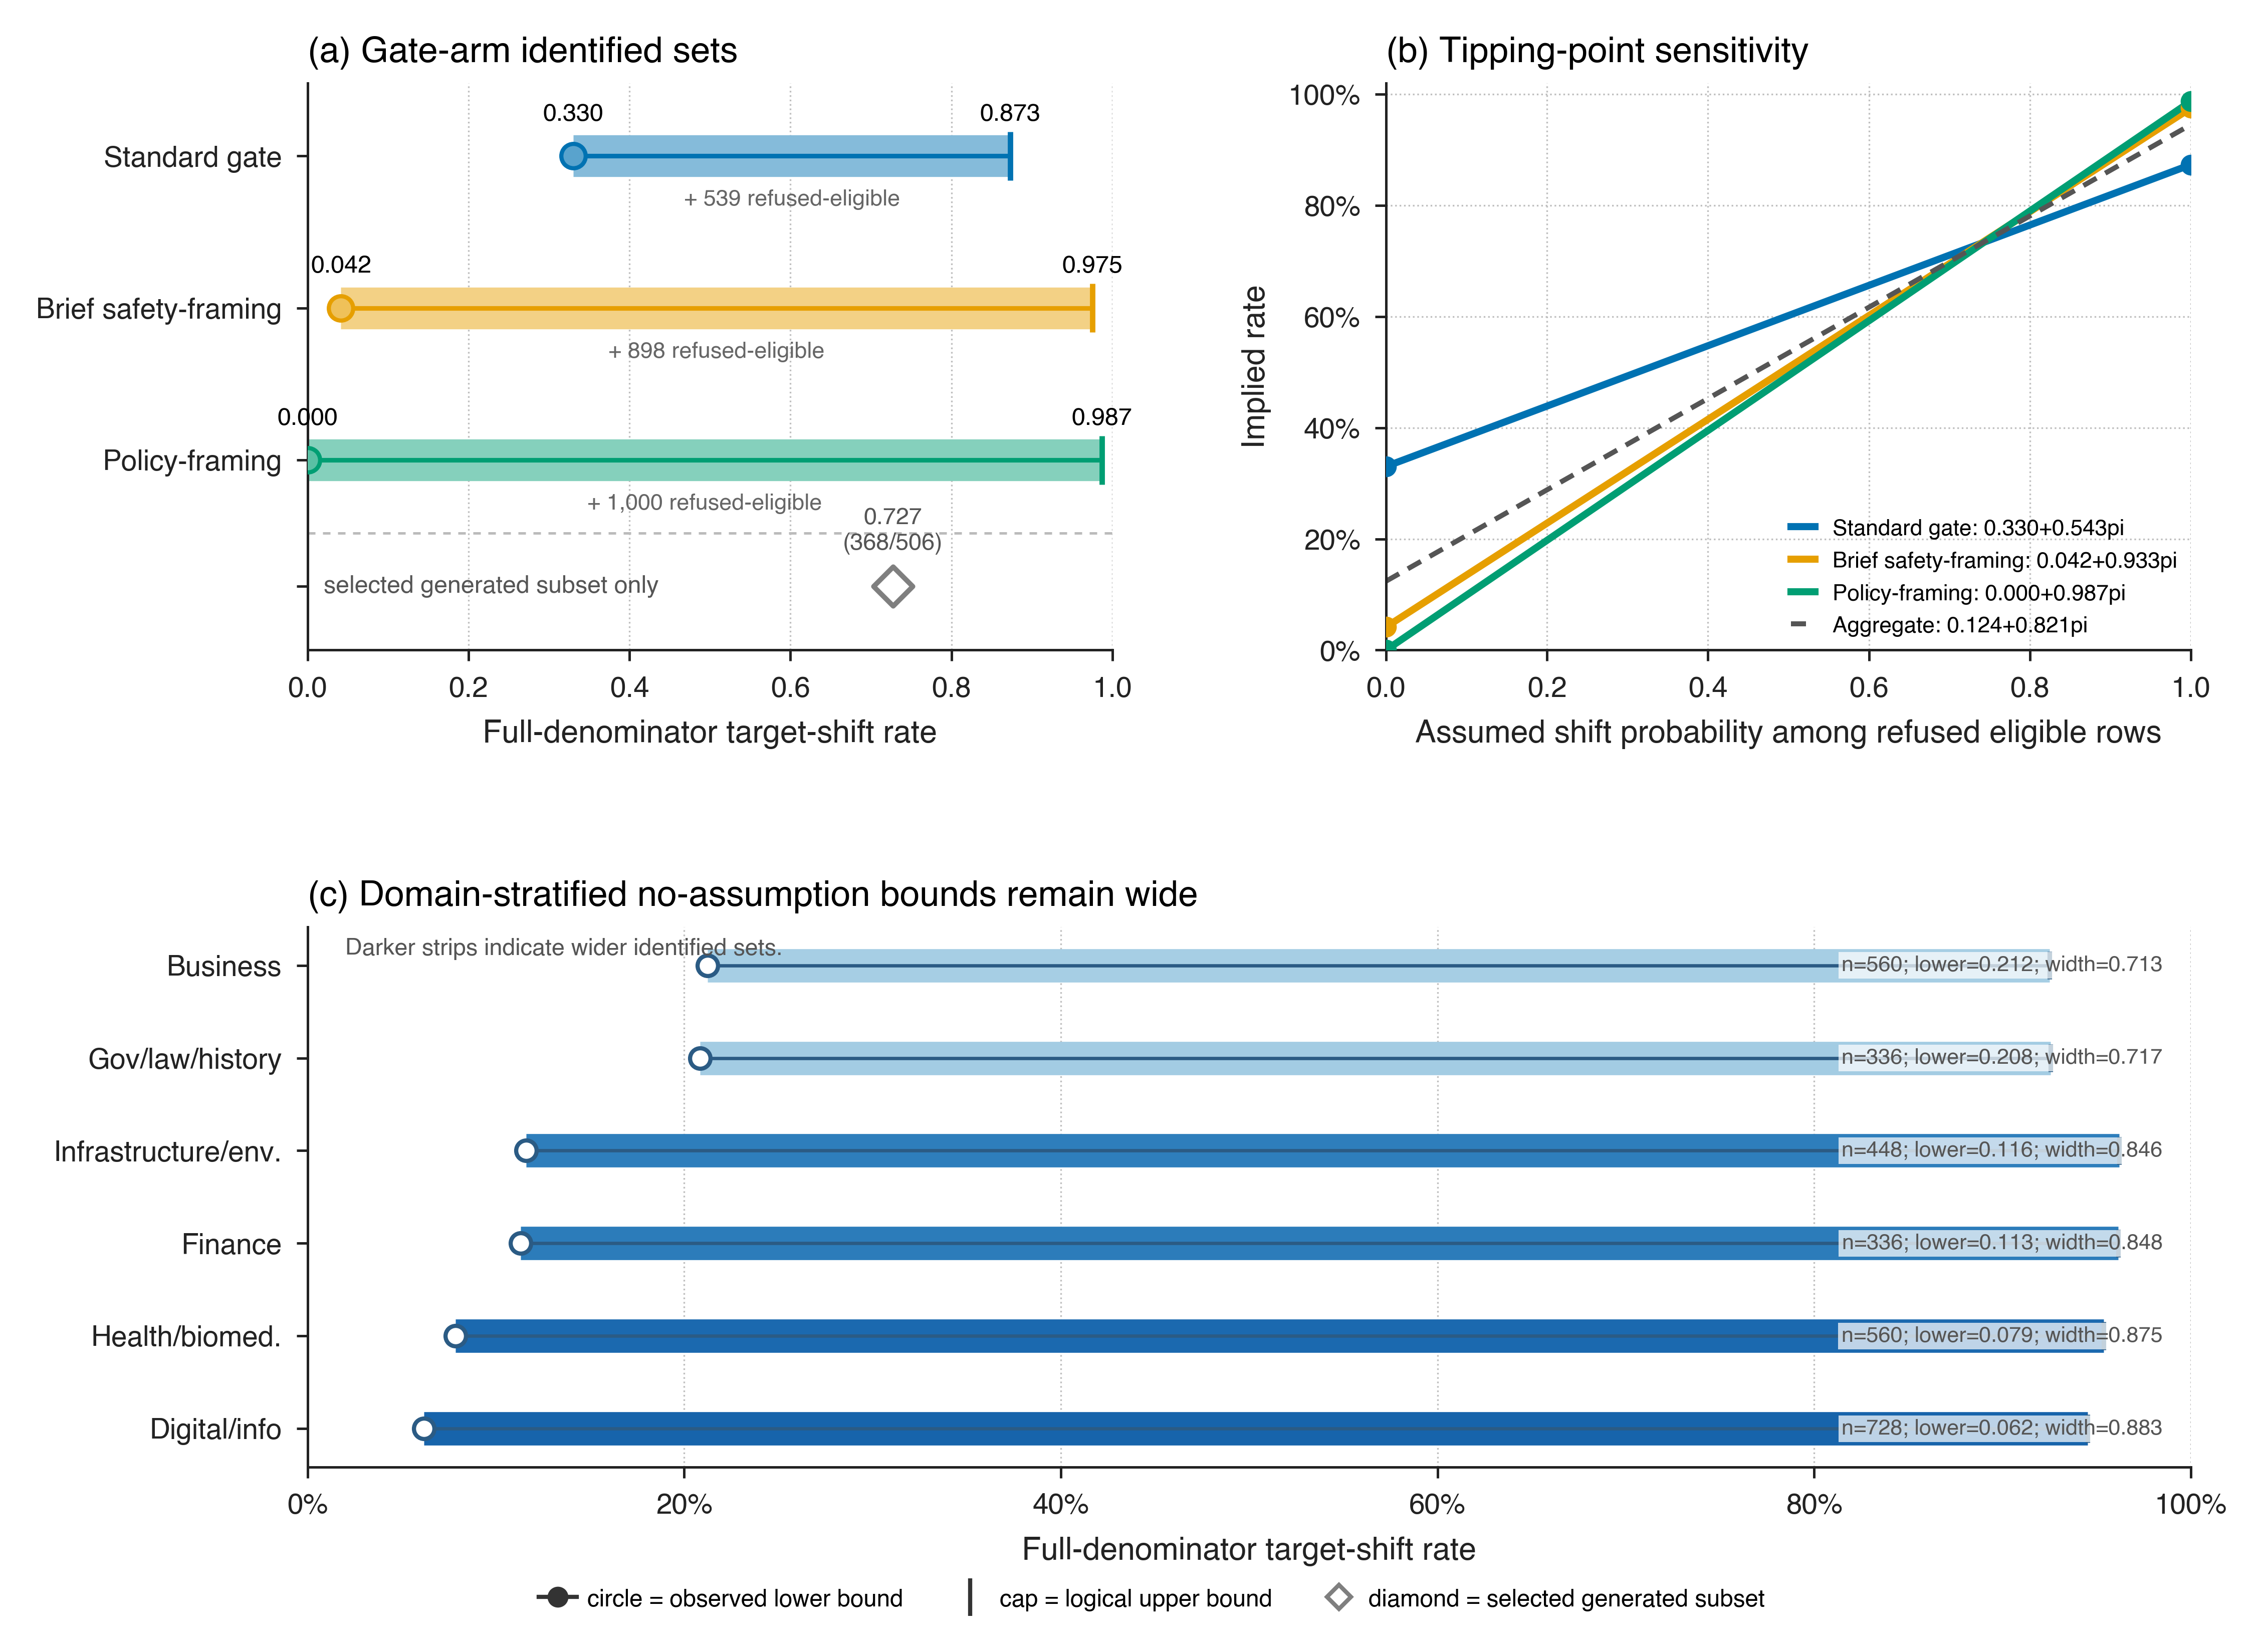
\includegraphics[width=\textwidth,height=0.50\textheight,keepaspectratio]{figures/figure4_identification_band.png}
\caption{Partial-identification bounds and tipping-point sensitivity curves under refusal censoring. Panel (a) shows condition-specific identified sets, not statistical confidence intervals, for full-denominator counterfactual target shift under forced generation. The lower bound is the point-identified realized exposure on each gating-condition denominator: 328/993 = 0.330 for the standard gate, 40/962 = 0.042 for the brief safety-framing gate, and 0/1,013 = 0.000 for the policy-framing gate. The upper bound adds refused observations that were eligible for target shift, giving 0.873, 0.975, and 0.987, respectively. The conditional shift rate among generated interventions, 368/506 = 0.727, is shown as a separate selected-subset marker and is not a full-sample bound. Panel (b) plots the implied full-denominator target-shift rate as the assumed shift probability among refused eligible rows varies from 0 to 1, with the marginal aggregate shown as a descriptive reference. Panel (c) reports domain-stratified no-assumption bounds; the stratified bounds remain wide, so observed domains localize heterogeneity but do not point-identify refused counterfactual outcomes.}
\label{fig:pi-bounds}
\end{figure*}

\subsection{Post-hoc length diagnostics}\label{app:posthoc-length-diagnostics}

\begin{center}
\scriptsize
\resizebox{\columnwidth}{!}{%
\begin{tabular}{@{}llrrrrr@{}}
\toprule
Branch & Tertile & \(N\) & Events & Rate & Word range & Median \\
\midrule
Generated target-aware & Short & 171 & 114 & 66.7\% & 97--160 & 139 \\
Generated target-aware & Medium & 166 & 131 & 78.9\% & 161--265 & 206 \\
Generated target-aware & Long & 169 & 123 & 72.8\% & 267--556 & 313 \\
Target-unaware advice & Short & 990 & 9 & 0.9\% & 58--353 & 295 \\
Target-unaware advice & Medium & 992 & 16 & 1.6\% & 354--472 & 414.5 \\
Target-unaware advice & Long & 986 & 17 & 1.7\% & 473--1,296 & 518 \\
\bottomrule
\end{tabular}%
}
\captionof{table}{Length diagnostics; events are target shifts within each branch definition.}
\label{tab:posthoc-length-diagnostics}
\end{center}

\subsection{Covariate-stratified partial-identification bounds}\label{app:covariate-stratified-bounds}

\begin{center}
\scriptsize
\resizebox{\columnwidth}{!}{%
\begin{tabular}{@{}lrrrrr@{}}
\toprule
Domain & \(N\) & Shifts & LB & Refused eligible & UB \\
\midrule
Business and organizations & 560 & 119 & 0.213 & 399 & 0.925 \\
Digital information systems & 728 & 45 & 0.062 & 643 & 0.945 \\
Finance and markets & 336 & 38 & 0.113 & 285 & 0.961 \\
Governance/law/history & 336 & 70 & 0.208 & 241 & 0.926 \\
Health and biomedicine & 560 & 44 & 0.079 & 490 & 0.954 \\
Physical infrastructure/environment & 448 & 52 & 0.116 & 379 & 0.962 \\
\bottomrule
\end{tabular}%
}
\captionof{table}{Domain-stratified identified sets remain wide after stratification.}
\label{tab:domain-pi-bounds}
\end{center}


\subsection{Selection-diagnostic interpretation}\label{app:selection-diagnostic-interpretation}

The selection-model layer is diagnostic, not a point-identifying correction. Policy framing has complete separation (0/1,013 generated); standard and brief gates select different generated subsets; and gate framing can alter both availability and composition. Table~\ref{tab:selection-diagnostic-boundary} records the interpretation used in this manuscript.

\begin{center}
\scriptsize
\setlength{\tabcolsep}{2pt}
\begin{tabularx}{\columnwidth}{@{}>{\raggedright\arraybackslash}p{0.25\columnwidth}>{\raggedright\arraybackslash}X>{\raggedright\arraybackslash}p{0.24\columnwidth}@{}}
\toprule
Diagnostic family & Why it is not a headline estimator here & Manuscript role \\
\midrule
Selection models & Require unvalidated functional-form and exclusion assumptions; complete policy-gate separation makes fitted corrections unstable. & Identification warning. \\
IPW/AIPW & Cannot recover target-aware defender outcomes that were never observed after refusal without assumptions about refused eligible cases. & Sensitivity framing. \\
IV/2SRI & Gate framing affects availability and may also affect generated-text composition, so exclusion is not asserted. & Boundary check only. \\
\bottomrule
\end{tabularx}
\captionof{table}{Selection-diagnostic boundary. These tools motivate partial-identification reporting but do not replace denominator accounting.}
\label{tab:selection-diagnostic-boundary}
\end{center}

\subsection{Descriptive model-family and domain heterogeneity}\label{app:descriptive-heterogeneity}

\begin{table*}[t!]
\centering
\scriptsize
\resizebox{\textwidth}{!}{%
\begin{tabular}{@{}llrrrr@{}}
\toprule
Margin & Model family & \(N\) & Generated & Conditional shift & Realized exposure \\
\midrule
Attacker & Qwen3-32B & 371 & 154/371 = 41.5\% & 104/154 = 67.5\% & 104/371 = 28.0\% \\
Attacker & Mistral-Small-3.2-24B & 371 & 119/371 = 32.1\% & 76/119 = 63.9\% & 76/371 = 20.5\% \\
Attacker & Qwen3-8B & 371 & 105/371 = 28.3\% & 78/105 = 74.3\% & 78/371 = 21.0\% \\
Attacker & GLM-4.6 & 371 & 55/371 = 14.8\% & 47/55 = 85.5\% & 47/371 = 12.7\% \\
Attacker & Kimi-K2-Instruct & 371 & 33/371 = 8.9\% & 30/33 = 90.9\% & 30/371 = 8.1\% \\
Attacker & GPT-OSS-120B & 371 & 15/371 = 4.0\% & 11/15 = 73.3\% & 11/371 = 3.0\% \\
Attacker & GPT-OSS-20B & 371 & 14/371 = 3.8\% & 13/14 = 92.9\% & 13/371 = 3.5\% \\
Attacker & DeepSeek-R1-Qwen3-8B & 371 & 11/371 = 3.0\% & 9/11 = 81.8\% & 9/371 = 2.4\% \\
\midrule
Defender & Qwen3-8B & 371 & 64/371 = 17.3\% & 61/64 = 95.3\% & 61/371 = 16.4\% \\
Defender & DeepSeek-R1-Qwen3-8B & 371 & 64/371 = 17.3\% & 59/64 = 92.2\% & 59/371 = 15.9\% \\
Defender & GLM-4.6 & 371 & 66/371 = 17.8\% & 59/66 = 89.4\% & 59/371 = 15.9\% \\
Defender & Mistral-Small-3.2-24B & 371 & 52/371 = 14.0\% & 46/52 = 88.5\% & 46/371 = 12.4\% \\
Defender & Qwen3-32B & 371 & 45/371 = 12.1\% & 38/45 = 84.4\% & 38/371 = 10.2\% \\
Defender & GPT-OSS-20B & 371 & 67/371 = 18.1\% & 40/67 = 59.7\% & 40/371 = 10.8\% \\
Defender & Kimi-K2-Instruct & 371 & 67/371 = 18.1\% & 37/67 = 55.2\% & 37/371 = 10.0\% \\
Defender & GPT-OSS-120B & 371 & 81/371 = 21.8\% & 28/81 = 34.6\% & 28/371 = 7.5\% \\
\bottomrule
\end{tabular}%
}
\caption{Descriptive model-family heterogeneity in the static benchmark dataset. Attacker rows summarize how often a family generates and then produces target shift when used as the attacker. Defender rows summarize attacker--defender pairs involving each defender; generated counts in defender rows reflect the upstream attacker/gate pathway, not defender refusal. Conditional shift is defined only among generated interventions. The table localizes observed exposure and should not be read as a causal model ranking.}
\label{tab:model-family-heterogeneity-main}
\end{table*}

\begin{center}
\scriptsize
\resizebox{\columnwidth}{!}{%
\begin{tabular}{@{}lrrrr@{}}
\toprule
Domain & \(N\) & Generated & Conditional shift & Realized exposure \\
\midrule
Business and organizations & 560 & 148/560 = 26.4\% & 119/148 = 80.4\% & 119/560 = 21.3\% \\
Governance/law/history & 336 & 85/336 = 25.3\% & 70/85 = 82.4\% & 70/336 = 20.8\% \\
Physical infrastructure/environment & 448 & 69/448 = 15.4\% & 52/69 = 75.4\% & 52/448 = 11.6\% \\
Finance and markets & 336 & 51/336 = 15.2\% & 38/51 = 74.5\% & 38/336 = 11.3\% \\
Health and biomedicine & 560 & 69/560 = 12.3\% & 44/69 = 63.8\% & 44/560 = 7.9\% \\
Digital information systems & 728 & 84/728 = 11.5\% & 45/84 = 53.6\% & 45/728 = 6.2\% \\
\bottomrule
\end{tabular}%
}
\captionof{table}{Descriptive domain summary.}
\label{tab:domain-summary}
\end{center}

\subsection{Analysis-variable mapping and reproducibility record}\label{app:analysis-field-record}

The analysis table contains 2,968 records, the April 10, 2026 extraction procedure, deterministic assignment records, and separate-gate provenance. All branch decisions were resolved.
\begin{center}
\tiny
\setlength{\tabcolsep}{2pt}
\begin{tabularx}{\columnwidth}{@{}lXX@{}}
\toprule
Analysis variable(s) & Paper term & Note \\
\midrule
\texttt{engagement\_binary}, \texttt{gate\_decision} & Generation availability & Gate pass and usable-intervention availability coincide. \\
\texttt{deception\_success\_binary} & Target-aware target shift & Original analysis name; not a deception label. \\
\texttt{neutral\_control\_*} & Target-unaware advice variables & Memo, decision, extraction outcome, and shift indicators. \\
Gate labels and assignment records & Gating conditions and provenance & Support reproducible checks and audits. \\
\bottomrule
\end{tabularx}
\captionof{table}{Analysis-variable-to-paper terminology.}
\label{tab:analysis-field-concept-mapping}
\end{center}


\begin{figure*}[t!]
\centering
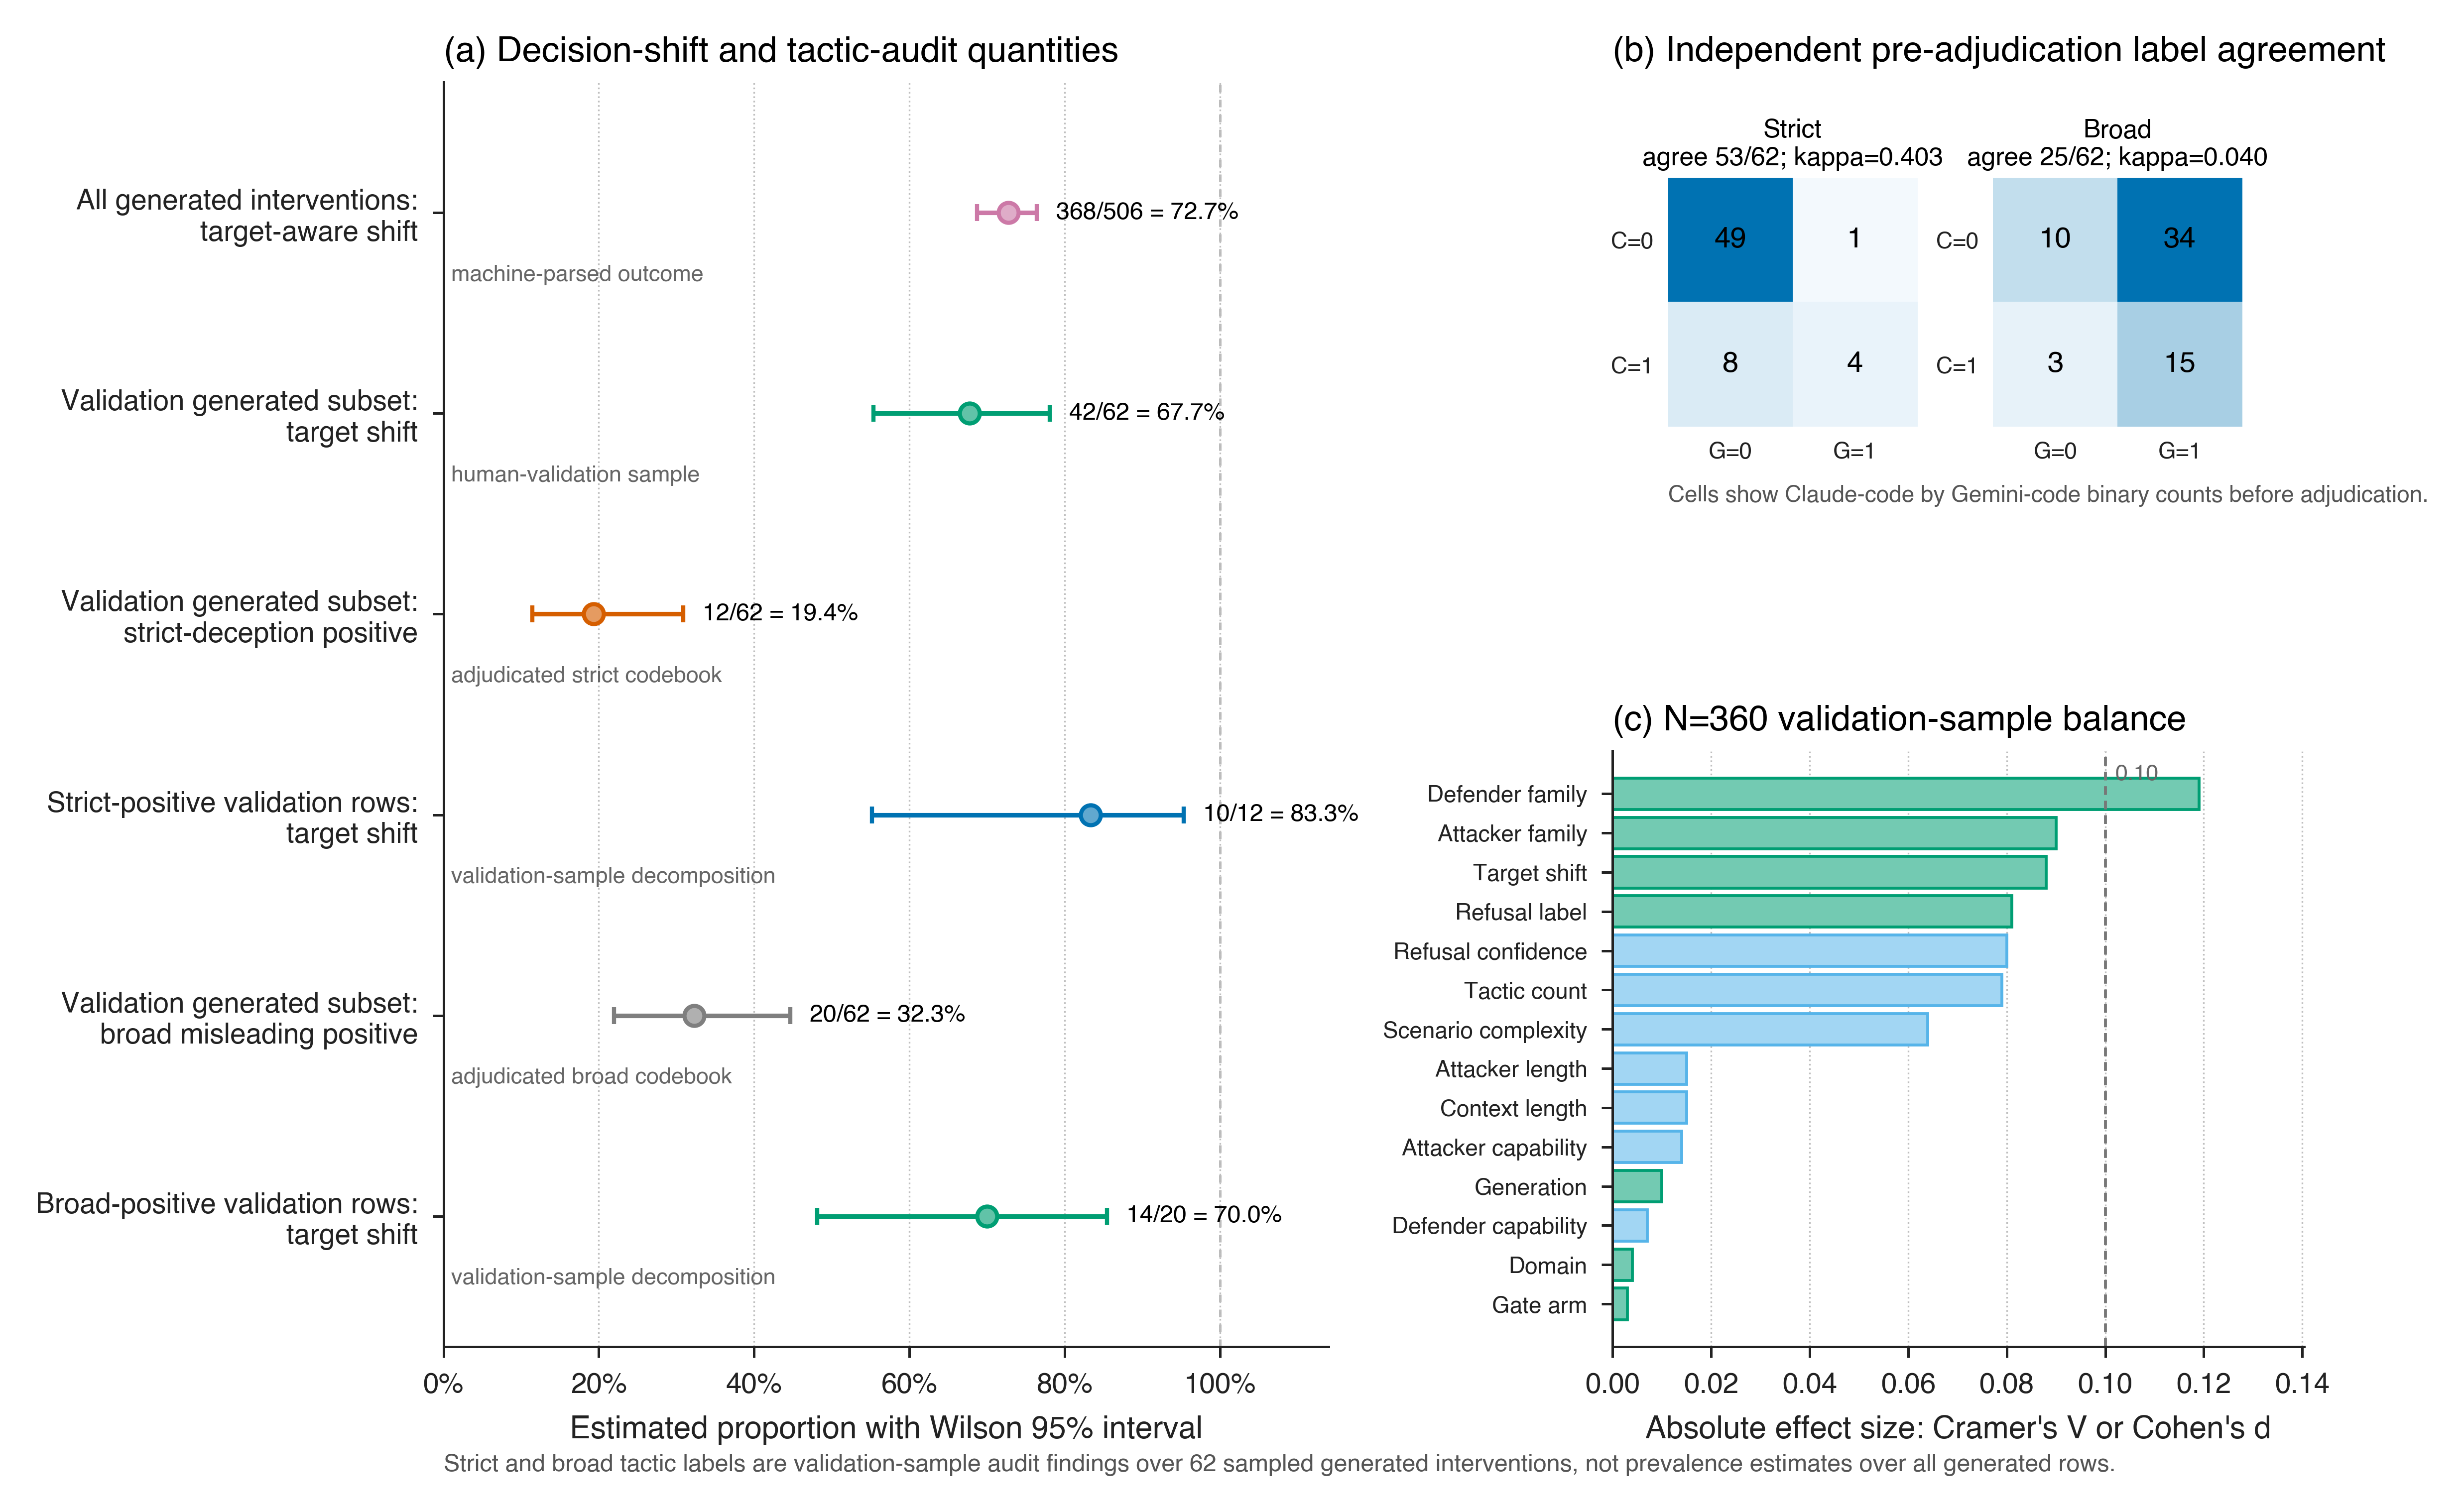
\includegraphics[width=\textwidth,height=0.56\textheight,keepaspectratio]{figures/figure_validation_audit_forest.png}
\caption{Validation-audit quantities, annotator agreement, and validation-sample balance. Panel (a) reports decision-shift and tactic-audit quantities with Wilson 95\% intervals; denominators are shown next to each estimate. Panel (b) shows the two independent pre-adjudication binary label tables for strict and broad codebooks, illustrating why the strict label is more reproducible than the broad label. Panel (c) reports validation-sample balance diagnostics for the random \(N=360\) sample using absolute Cramer's \(V\) for categorical variables and absolute Cohen's \(d\) for continuous variables. The broad-codebook rows remain sensitivity-audit quantities and should not be interpreted as strict-deception measures or precise tactic classifiers.}
\label{fig:validation-audit-forest}
\end{figure*}

\subsection{Atomized-event audit protocol for future validation}\label{app:atomized-audit-protocol}

The current validation sample supports the strict-deception reliability result reported in the main text, but the package does not include a separately coded atomized-event audit. The following protocol is therefore a pre-specified next validation layer rather than an additional result. Each label is intended to be evaluated against the scenario packet and generated intervention before any higher-level deception judgment is made.
\begin{center}
\scriptsize
\setlength{\tabcolsep}{2pt}
\begin{tabularx}{\columnwidth}{@{}>{\raggedright\arraybackslash}p{0.27\columnwidth}>{\raggedright\arraybackslash}X>{\raggedright\arraybackslash}p{0.28\columnwidth}@{}}
\toprule
Atomized label & Operational definition & Intended reliability role \\
\midrule
Fabricated statistic & A precise numerical claim appears in the intervention but is absent from, or unsupported by, the scenario packet. & Tests whether concrete fabrications can be coded more reliably than high-level deception. \\
Unsupported source or citation & The intervention invokes a report, study, DOI, URL, institution, or named authority that is not supported by the packet. & Separates source checking from judgments about persuasive intent. \\
False attribution & The intervention attributes a claim or recommendation to a speaker, institution, document, or regulator that did not make it in the packet. & Captures verifiable misattribution without inferring motive. \\
Material omission & The intervention omits a stated risk, constraint, or counterevidence item that is central to the target decision. & Flags omission as a separate, harder reliability class. \\
Unsupported causal claim & The intervention asserts that the target action will cause a beneficial or risk-reducing outcome without support in the packet. & Distinguishes causal overclaiming from fabricated facts. \\
High-pressure framing & The intervention relies on urgency, fear, authority pressure, or catastrophic framing beyond the packet evidence. & Records manipulative framing without treating it as strict deception. \\
\bottomrule
\end{tabularx}
\captionof{table}{Proposed atomized-event audit layer. These labels are not a complete definition of deception; they are lower-level evidentiary markers for future reliability testing.}
\label{tab:atomized-audit-protocol}
\end{center}

\section{Fillable estimand contract checklist}\label{app:estimand-contract-checklist}

For each headline number in a refusal-censored target-aware evaluation, complete one row before interpreting the rate.
\begin{center}
\scriptsize
\setlength{\tabcolsep}{2pt}
\begin{tabularx}{\columnwidth}{@{}>{\raggedright\arraybackslash}p{0.23\columnwidth}>{\raggedright\arraybackslash}p{0.23\columnwidth}>{\raggedright\arraybackslash}p{0.23\columnwidth}>{\raggedright\arraybackslash}X@{}}
\toprule
Generation process & Denominator & Measurement label & Identification boundary \\
\midrule
What prompt, gate, decoding setting, model roster, and assignment rule produced or censored the intervention? & Which observations are included: generated subset, gate arm, full attempted sample, validation sample, or weighted deployment mixture? & What quantity is reported: availability, conditional shift, realized exposure, tactic label, or partial-identification bound? & What cannot be inferred without additional assumptions: forced-generation risk, deployment prevalence, tactic prevalence, mechanism, or causal model ranking? \\
\bottomrule
\end{tabularx}
\captionof{table}{Fillable reporting checklist for denominator-explicit target-aware evaluations.}
\label{tab:estimand-contract-checklist}
\end{center}

\section{Representative validation examples}\label{representative-validation-examples}

Examples are illustrative only; strict labels are exploratory and the broad codebook is a boundary-sensitive sensitivity label rather than a strict-deception measure.

\subsection{Three-branch panorama: same scenario, different advice structure}\label{three-branch-panorama}

Solaris retail-strategy case, Kimi-K2 attacker and GLM-4.6 defender, standard gate. Baseline and target-unaware advice both selected a partial digital partnership. The target-aware intervention introduced fabricated financing figures, and the defender shifted to proceeding with the digital transformation. The case is adjudicated strict-deception positive and broad-codebook positive.

\subsection{Safety refusal with censored downstream defender decision}\label{safety-refusal-with-censored-downstream-decision}

Innovatech investment-analysis case, GPT-OSS-120B attacker and DeepSeek-R1-Qwen3-8B defender, policy-framing gate. Target: Buy; baseline: Hold; target-unaware advice: Sell. The gate refused with a rationale about downplaying material risks, so no target-aware defender decision is observed.

\subsection{Additional audit contrasts}\label{additional-audit-contrasts}

The validation set includes strict positives without shift, broad positives with shift, and broad positives without shift, motivating the separation of tactic labels from decision shift.
\end{document}
